\documentclass[12pt,english,a4paper]{report}

\usepackage[utf8]{inputenc}          % Allows UTF-8 encoded characters in the .tex-file.
\usepackage{babel,csquotes,textcomp,duomasterforside} % Set LaTeX to structure the content following international academic standards.

\usepackage[toc,page]{appendix}

\usepackage{hyperref}
\usepackage{graphicx}
\usepackage{pdfpages}
\usepackage{listings}
\usepackage{wrapfig}
\usepackage{color,colortbl}
\usepackage{lettrine}
\usepackage[font={small,it}]{caption}
\usepackage{multirow}
\usepackage{tabularx}
\usepackage{footnote}
\usepackage{subfiles}
\usepackage{minted}
\usepackage{fancyvrb}
\usepackage{lscape}
\usepackage{tabularx}

\usemintedstyle{friendly}

\newmintedfile[pythoncode]{python}{
fontsize=\scriptsize,
fontfamily=tt,
linenos=true,
numberblanklines=true,
numbersep=12pt,
numbersep=5pt,
gobble=0,
frame=leftline,
framerule=0.4pt,
framesep=2mm,
funcnamehighlighting=true,
tabsize=4,
obeytabs=false,
mathescape=false
samepage=false, %with this setting you can force the list to appear on the same page
showspaces=false,
showtabs =false,
texcl=false,
%breaklines = true
}

\newmintedfile[ccode]{c}{
fontsize=\scriptsize,
fontfamily=tt,
linenos=true,
numberblanklines=true,
numbersep=12pt,
numbersep=5pt,
gobble=0,
frame=leftline,
framerule=0.4pt,
framesep=2mm,
funcnamehighlighting=true,
tabsize=4,
obeytabs=false,
mathescape=false
samepage=false, %with this setting you can force the list to appear on the same page
showspaces=false,
showtabs =false,
texcl=false,
%breaklines = true
}

\newmintedfile[makecode]{make}{
fontsize=\scriptsize,
fontfamily=tt,
linenos=true,
numberblanklines=true,
numbersep=12pt,
numbersep=5pt,
gobble=0,
frame=leftline,
framerule=0.4pt,
framesep=2mm,
funcnamehighlighting=true,
tabsize=4,
obeytabs=false,
mathescape=false
samepage=false, %with this setting you can force the list to appear on the same page
showspaces=false,
showtabs =false,
texcl=false,
%breaklines =true
}

% Making the whole paragraph biz possible
%\usepackage{titlesec}
%\setcounter{secnumdepth}{4}
%\titleformat{\paragraph}
%{\normalfont\normalsize\bfseries}{\theparagraph}{1em}{}
%\titlespacing*{\paragraph}
%{0pt}{3.25ex plus 1ex minus .2ex}{1.5ex plus .2ex}

% Adding the bib
\usepackage[
    backend=biber,
    style=numeric
]{biblatex}
\addbibresource{refs.bib}

\definecolor{mygreen}{rgb}{0,0.6,0}
\definecolor{mygray}{rgb}{0.5,0.5,0.5}
\definecolor{mymauve}{rgb}{0.58,0,0.82}
\definecolor{auxiliryc}{RGB}{70,240,161} %Green
\definecolor{ineffectivec}{RGB}{70,149,240} %purple
\definecolor{effectivec}{RGB}{115,70,240} % Blue

\graphicspath{{./graphics/}}

% Setting tty font?
%\lstset{ %
%  basicstyle=\ttfamily\small,     
%  backgroundcolor=\color{white},   % choose the background color
%  breaklines=true,                 % automatic line breaking only at whitespace
%  captionpos=b,                    % sets the caption-position to bottom
%  commentstyle=\color{mygreen},    % comment style
%  escapeinside={\%*}{*)},          % if you want to add LaTeX within your code
%  keywordstyle=\color{blue},       % keyword style
%  stringstyle=\color{mymauve},     % string literal style
%  showspaces=false,
%  showstringspaces=false,
%}

\lstset{language=C,
  basicstyle=\ttfamily\scriptsize,
  keywordstyle=\color{blue}\ttfamily,
  stringstyle=\color{red}\ttfamily,
  commentstyle=\color{green}\ttfamily,
  breaklines=true,
  showspaces=false,
  showstringspaces=false,
  numbers=left,                    % where to put the line-numbers; possible values are (none, left, right)
  numbersep=5pt,    
  frame=single,                 % how far the line-numbers are from the code
  numberstyle=\tiny\color{mygray}, % the style that is used for the line-numbers
  rulecolor=\color{black}         % if not set, the frame-color may be changed on line-breaks 
}

\newenvironment{code}{\captionsetup{type=listing}}{}

\title{GPS Time Spoofing}
\subtitle{A detection and mitigation system for GPS timing}
\author{Aril Schultzen}
\begin{document}
\duoforside[dept={Institutt for informatikk},
program={Informatikk: programmering og nettverk},
long]

\begin{abstract}
Abstract goes here.
\end{abstract}

\chapter*{Foreword}
Here goes foreword

% Hackish code to keep counters and white pages at bay
\thispagestyle{empty}
\setcounter{page}{0}
\tableofcontents
\thispagestyle{empty}
\setcounter{page}{0}
\thispagestyle{empty}
\setcounter{page}{0}
\clearpage
\setcounter{page}{1}

% Here goes all the chapters
% ==================================================

\subfile{intro}

% Chapter about the csac and it's connectivity?

\chapter{Hardware}

\section{Chip Scale Atomic Clock}
I propose to use the Symmetricom SA.45 as the CSAC. This is a CSAC measuring only 16cc with 1 pulse per second (PPS) output and 1 PPS input (for disciplining). The SA.45's strength is it's low power consumption (less than 120mW) and low price \cite{SADS}. The SA.45 also uses a built-in controller which can be communicated with over a RS-232 serial interface. The ability to communicate with the CSAC, issue commands and collect data, is paramount for the feasibility of our proposal. It's worth mentioning that any atomic clock such as Cesium standard or even a Rubidium standard could be used given that they have a means to communicate basic telemetry as used by the SMACC software.

\section{SMACC platform}
I propose to use the Raspberry Pi 3 Model B (RASPI3) in the role as the host running the SMACC software. The RASPI3 is an interesting piece of equipment with an impressive list of specifications. It is a single board computer with a 1.2GHz 64-bit quad-core ARMv8 CPU, 1 GB of RAM, built in 802.11n Wireless LAN and four USB ports (\cite{RASPI}) (just to mention some). As with the Symmetricom SA.45, the RASPI3 is very affordable and retailed at about 35 USD when this report was written. We also propose to use Raspbian (\cite{RASPBIAN}), a Debian derived flavor of Linux optimized for the Raspberry Pi as the operating system. 

\section{GNSS receiver}
I propose to use at least two GNSS receivers. Both of the receivers should simply collect data and feed it to the SMACC but one of the receivers should also double as a 1 PPS disciplining source for the CSAC. Considering that need for a stable 1 PPS source, I propose to use the u-blox NEO-M8T. This is a relativity affordable GNSS receiver with a temperature compensated crystal oscillator (TCXO), 3 concurrent GNSS reception and an external antenna (\cite{UBLOXM8T}). Currently, only strings of NMEA data is collected from the GNSS receiver. However in the future it might be beneficial to collect and process raw data from the receivers as well. Since most GNSS receivers today follow the NMEA standard (to some extent) and raw data currently isn't required, common and popular receivers like the u-blox NEO-NEO series should be more that sufficient to use in an implementation if this proposal.

\chapter{Software}
\section{The Sensor Server/Client model}
Numerous approaches where considered when planning the implementation of the SMACC software (See \ref{da} for alternate approaches). The approach that was chosen is a Client/Server model which I have named the "Sensor Server". The Sensor Server model is based on the idea that a GNSS receiver and a computer can be viewed abstractly as a single device, a Sensor. The Server and Sensor communicates over an IP network. The Sensor runs a trivial program that receives data from a GNSS receiver, formats the data correctly and sends the data to a Server (more about the client \ref{sensor_client}). The Server on the other hand, is responsible for the heavy lifting. The data gathered from the Sensors are applied to what we call \textit{filters}. The filters are just algorithms that are able to detect anomalies in the data, thus making it possible to react to a spoofing or jamming attempt. Server tasks include:
\begin{itemize}
  \item Handle connections to all Sensors.
  \item Update structures as Sensor status changes (Disconnects, kick request)
  \item Communication with the CSAC and CSAC model updating
  \item Sensor data analysis and filter updates
  \item Raising alarms based on filter status
\end{itemize}
By using already existing network infrastructure, it becomes a lot easier to distribute Sensors and cover more area. This makes spoofing attacks harder to implement and easier to detect(\ref{cspakp}).However, every router and switch between a Sensor and the Server imposes a delay on the stream of packets between the two, especially when compared with a directly cabled approach. This might make the Sensor Server approach less responsive. It is of our understanding that whatever increase in complexity the Client/Server introduces to our approach, the Sensor Server makes up for by eliminating the need for potential miles of signal cables and signal amplifiers. 

\begin{figure}
\centering
  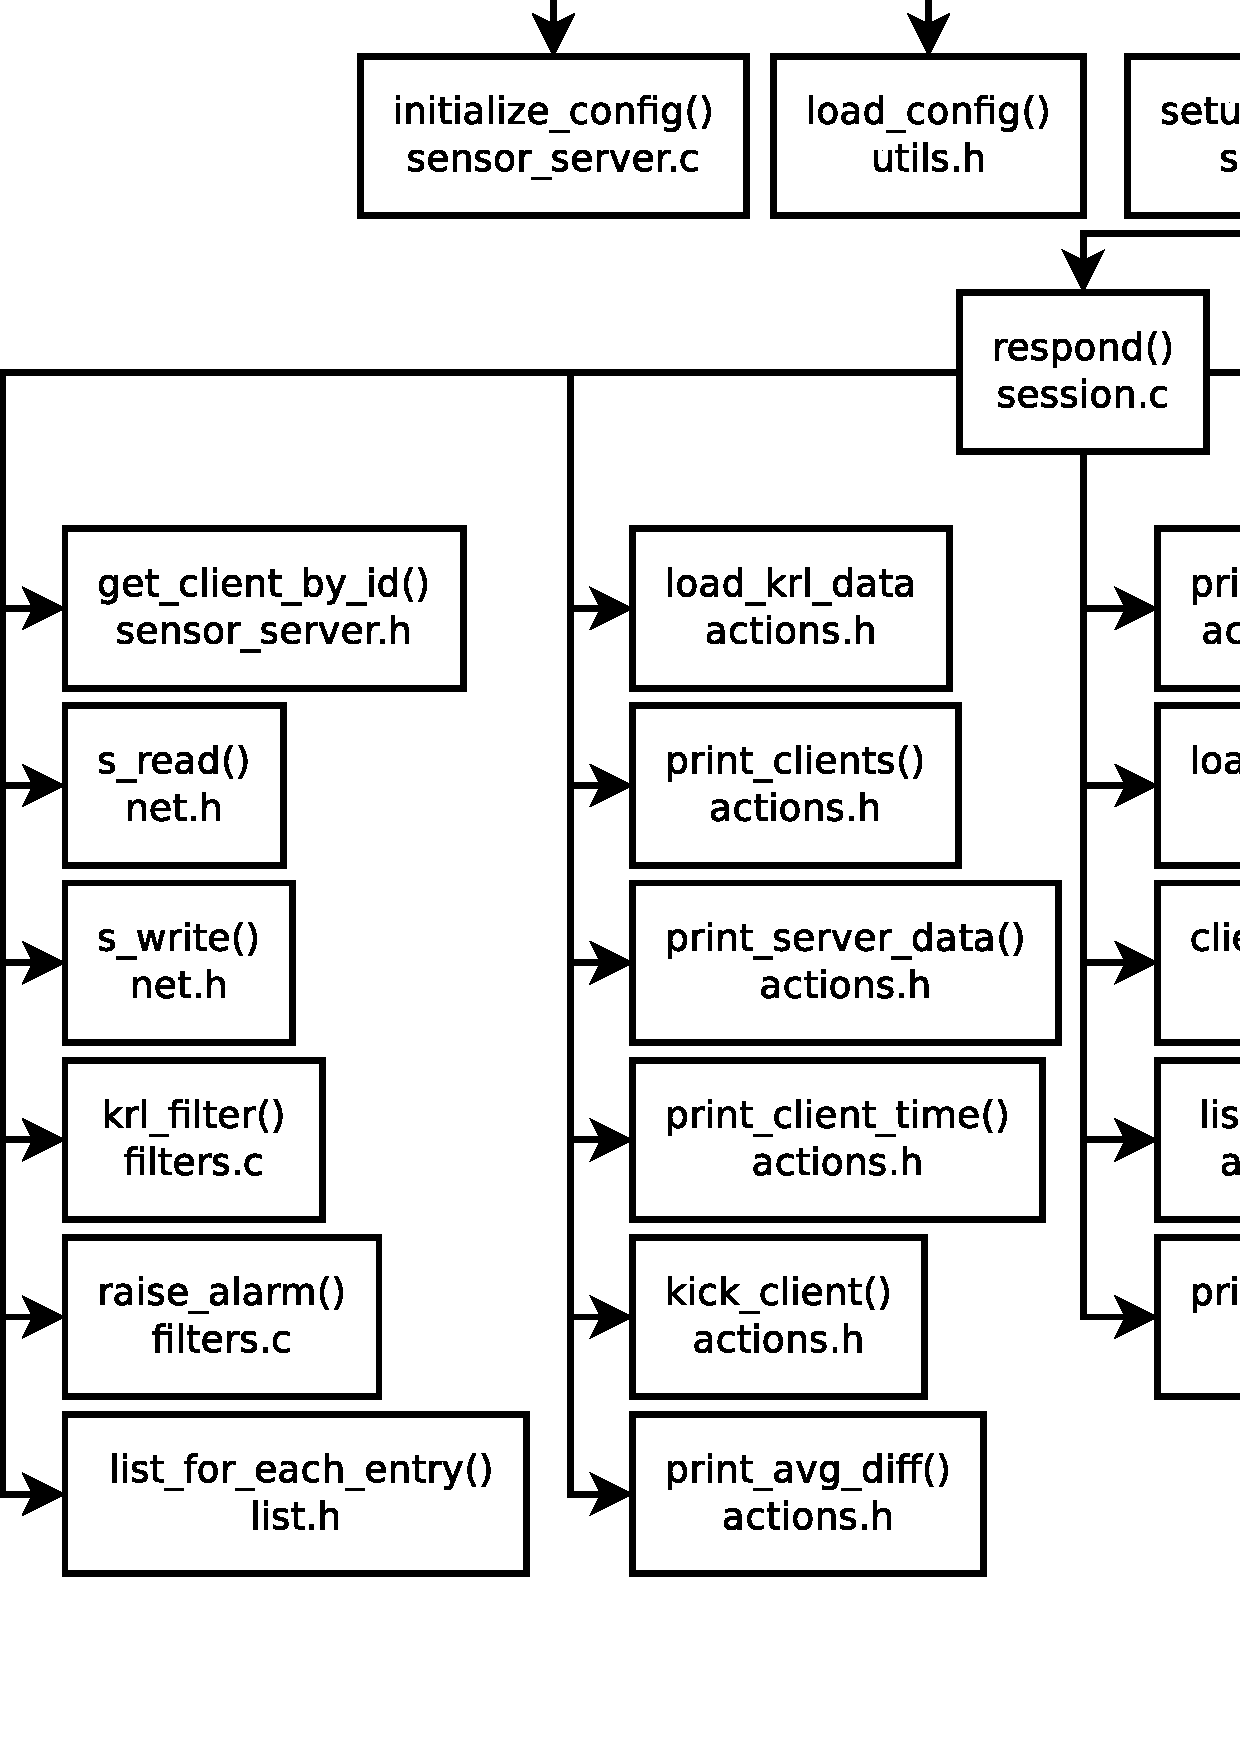
\includegraphics[scale=0.3]{server_call_graph.pdf}
   \caption[Sensor Server simplified call graph]{Simplified call graph for the Sensor Server.}
   \label{server_call_graph}
\end{figure}

\newpage
\subsection{Roles}\label{roles}
A client connected to the server can have two roles; It can either be a Sensor or a Monitor. The Sensor role is already explained, but the Monitor role was added in order for a user of the Sensor Server to connect to the server and check status or issue commands. For a client to assume the role of a Monitor, the client has to pick a negative integer as ID number. This way, the Server does not expect you as a client to report any NMEA data the way it would with a Sensor. The Monitor role can also be used to interface with the Server. See (\ref{interface}) for more.

\subsection{Sockets}\label{sockets}
In order to implement the Server/Client model, the Sensor Server and Sensor Client is implemented using the Linux Socket API. The API is based on BSD sockets and are available in in almost all Unix like operating system (\cite{LINUX_KERNEL}, p.610). Listing \ref{server_connect} shows a sample of code taken from one of the Sensor Server's source file. The sample shows the following:
\begin{itemize}
  \item Line 4: The server waits for a connection. \texttt{accept()} is a blocking function. The code does not continue past this point before a client has connected.  
  \item Line 12: The code has been executed way past the blocking \texttt{accept} function. Someone must have connected! The server forks out a new process from this point in the execution with the function \texttt{fork()}.
  \item Line 13: Upon entering the if statements regarding it's process identification (PID), the parent ends back at the top in the while loop. The child on the other hand, matches the criteria for the if sentence at line 15.
  \item Line 16: The child process closes it's parent's socket file descriptor and continues to setup the session at the next line.
\end{itemize}

\begin{code}
  \caption{Sample of code taken from \texttt{sensor\_server.c}(\ref{sensor_server.c}, line 356). The sample has been edited for clarity purposes.}
  \begin{minted}
  [
  fontsize=\footnotesize,
  fontfamily=tt,
  linenos=true
  ]
  {c}
    listen(server_sockfd,SOMAXCONN);
    int session_fd = 0;
    while (!done) {
        session_fd = accept(server_sockfd,0,0);
        if (session_fd==-1) {
            if (errno==EINTR) continue;
            t_print(ERROR_CONNECTION_ACCEPT,errno);
        }
        if(number_of_clients == max_clients) {
            close(session_fd);
        } else {
            pid_t pid=fork();
            if (pid==-1) {
                printf(ERROR_FAILED_FORK, errno);
            } else if (pid==0) {
                close(server_sockfd);
                setup_session(session_fd, new_client);
                close(session_fd);
                _exit(0);
            } else {
                close(session_fd);
            }
        }
    }
  \end{minted}
  \label{server_connect}
\end{code}
Even though the \texttt{accept()} function in the sockets API is blocking, CPU cycles are not wasted. If a socket call cannot be completed immediately, the process who issued the call will be put to sleep thus enabling the scheduler to schedule other processes for execution until conditions are right for the sleeping process. (\cite{UNIXN_WBA}, p.435). It is also possible to use non-blocking socket calls, and while this often increases performance, it also increases complexity, and was therefor not chosen for this approach. It's also worth mentioning that one could create \textit{threads} instead of forking out processes for new connections. The creation of threads are typically less expensive in terms of CPU cycles than the creation of processes. Processes on the other hand, always have their own virtual address space as opposed to threads who share their address space with the other threads withing the process. This makes programming with threads more complex and the result of a crash more severe as it affects the other threads as well. 

\subsection{Shared memory \& Semaphores}\label{shared_mem_sem}
As mentioned earlier (\ref{sockets}), every time a client connects, a new process is born to take care of the communication with the new client. Since every process has got it's own virtual address space, the processes are isolated from each other. This posed a challenge because we wanted the Sensor Server as a whole with all processes to be able to communicate with each other and share data and communicate. IPC (inter process communication) is nothing new, and one way to accomplish it, is to use shared memory segments. The sensor server architecture uses several shared memory segments. The pointers to the shared memory segments are declared as \textit{extern} in \texttt{sensor\_server.h}. The extern keyword means the the variable has an external linkage, making it visible from other files than the one in which it is defined. Listing \ref{extern_structs} shows a code sample taken from \texttt{sensor\_server.h} where the shared memory segments are declared.

\begin{code}
  \caption{Sample of code from \texttt{sensor\_server.h}(\ref{sensor_server.h}, line 356) where shared memory segments are declared.}
  \begin{minted}
  [
  fontsize=\footnotesize,
  fontfamily=tt,
  linenos=true
  ]
  {c}
    extern volatile sig_atomic_t done;
    extern struct client_table_entry *client_list;
    extern struct server_data *s_data;
    extern struct server_synchro *s_synch;
    extern struct server_config *s_conf;
    extern struct csac_filter_data *cfd;
  \end{minted}
  \label{extern_structs}
\end{code}

These shared memory segments have different usage. The \texttt{client\_list} points to a shared segment allocated for storing a list of all connected clients. \texttt{s\_data} contains information about the server, \texttt{s\_synch} contains semaphores used to lock down shared resources, \texttt{s\_conf} is the servers configuration and \texttt{cfd} is the CSAC filters data and state. Every process that forks out from the server is given access to these memory segment. One might make the point that this voids the idea of processes, and one might be correct (see \ref{discussion}). The shared memory is created using the GNU library's Memory Mapped I/O (MMAP). Although typically used to map files to a region of memory, MMAP can also be used to create an anonymous map which is not connected to file but rather for sharing data between tasks without using files.

\subsubsection{Client list memory segment}
Every time a client connects, it is given a piece of shared memory where it can store its data. This piece of is shared memory is used as a node in a linked list. The linked list structure, stored in the shared memory segment is available to all the processes spawned by the server. This segment is static in size and is allocated once and never changed during the whole life of the Server. The size of the segment is determined by the maximum number of allowed clients, a configurable value read from the configuration file every time the server is started. Ideally, the segment should be resize-able and the size should depend the amount of connected client. M. Kerrisk explains in his "The Linux Programming Interface" (\cite{kerrisk2010linux}), that most UNIX implementations does not support resizing of a memory map like the shared memory segments used in the Sensor Server. However, there is non-portable and Linux specific system call, \texttt{mremap()} that can be used on Linux system for this purpose. Unfortunately, the address returned by \texttt{mremap()} might be different from the old address to the shared memory segment. This would mean that pointer inside the shared segment might no longer be valid after a resize operation has been done. A way to avoid this problem caused by the remapping, would be to use offsets instead of pointers when referring to addresses in the mapped region. This would however increase the complexity of the server. The potential waste of memory would never be substantial when considering that the size of the \texttt{client\_table\_entry} struct is a mere 4664 bytes. This is why the current implementation with shared memory segment of static size was chosen.

\subsubsection{Using the client list memory segment}\label{create_client}
As previously explained, the list of clients are stored in a shared memory segment using a linked list structure. In order to keep tabs on what part of the shared memory segment is in use, a simple map of the memory is used(\ref{memory_map_figure}):
\begin{figure}
\centering
  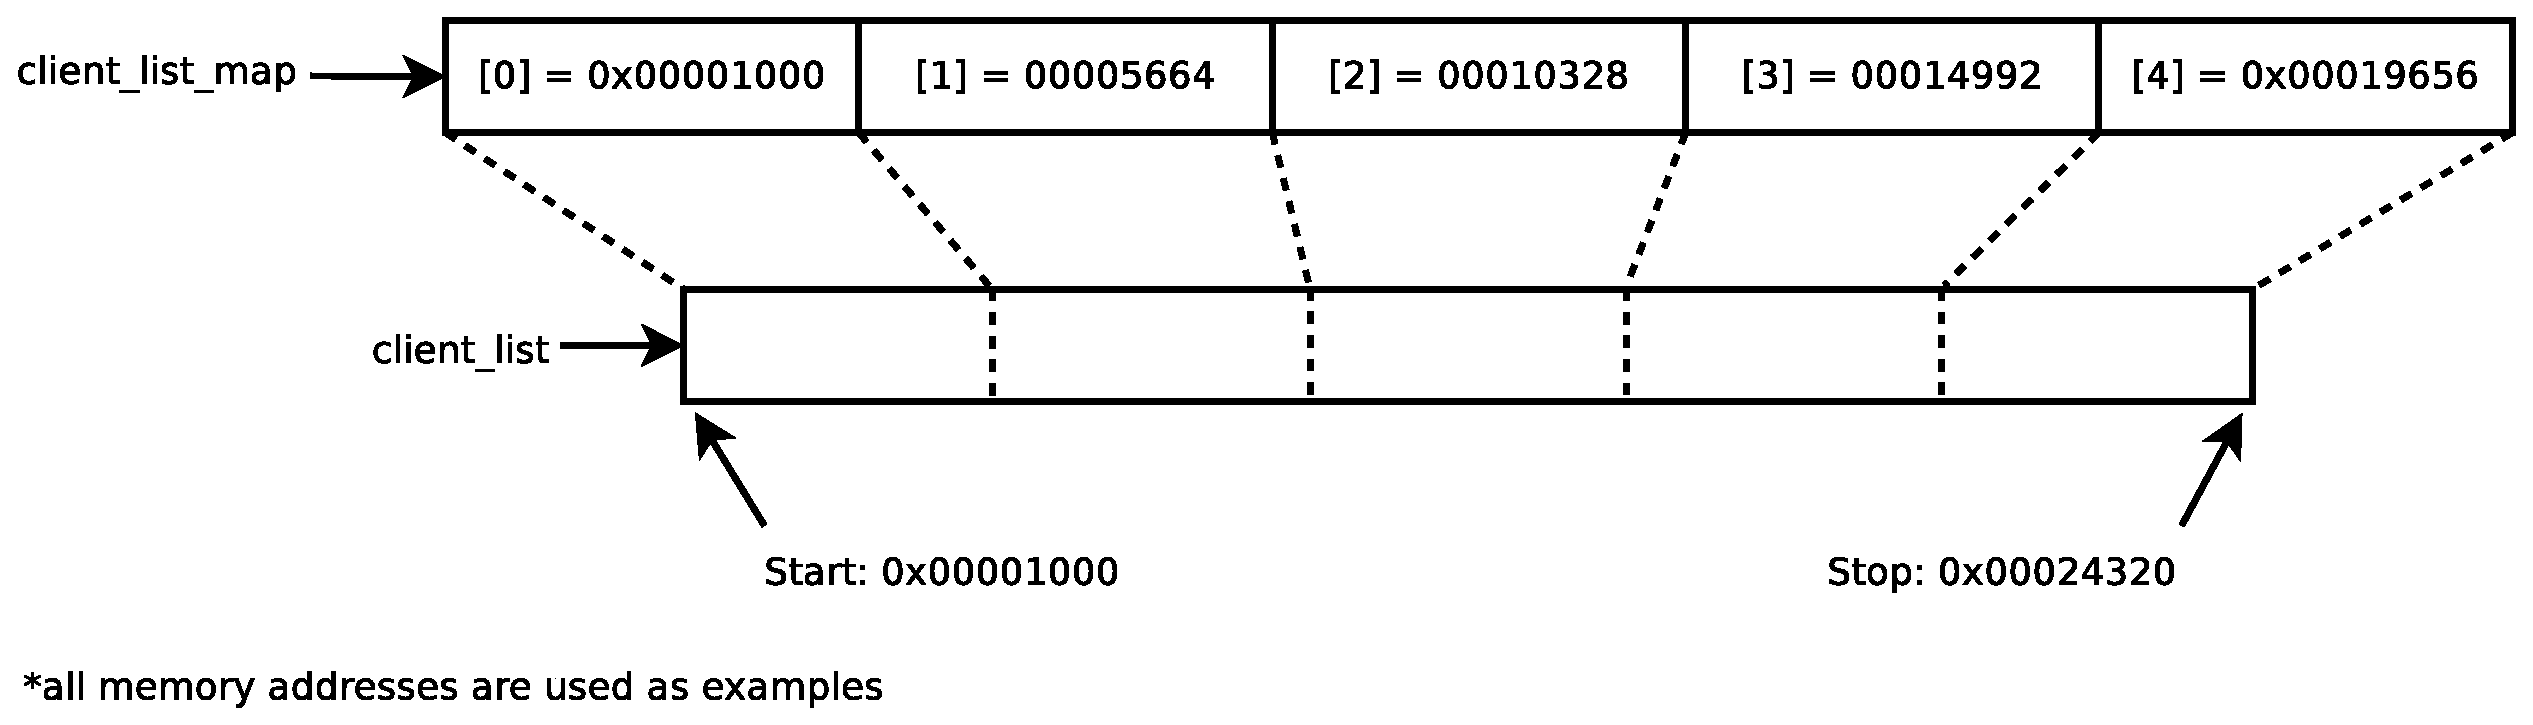
\includegraphics[scale=0.3]{mem_layout}
   \caption[Memory map layout example]{Figure is showing the relation between the shared memory segment containing the client list and the memory map}
   \label{memory_map_figure}
\end{figure} 

The map is an array containing pointers to the client list segment. These pointers are offset by the size of the \texttt{client\_table\_struct} and maps 1:1 to what can be thought of as individual \textit{pieces} of memory in the client list shared memory segment. A free piece of memory is in the map represented by a pointer that is not NULL. Figure \ref{get_mem_pieces} shows the function that iterates through the map to find a free piece. 

\begin{code}
  \caption{Sample of code showing the \texttt{get\_mem\_piece()} function.}
    \begin{minted}
    [
    fontsize=\footnotesize,
    fontfamily=tt,
    linenos=true
    ]
    {c}
    static struct client_table_entry* get_mem_piece()
    {
        int i;
        for(i = 1; i < s_conf->max_clients; i++){
            if(client_list_map[i] != NULL){
                struct client_table_entry *tmp = client_list_map[i];
                client_list_map[i] = NULL;
                return tmp;
            }
            i++;
        }
        return NULL;
    }
    \end{minted}
    \label{get_mem_piece}
\end{code}

\subsubsection{Client linked list}\label{linked_list}
Since the C standard does not provide data structures like linked lists, I had to choose between reinventing the wheel or finding some implementation to drop into the project. While studying another subject, I found a guide on how to use the linked list implementation from the linux kernel source code (\cite{KAZU_LIST}) in a user space program. Since the implementation was extremely solid, well tested and had many useful functions, i decided to use it. The modified header file containing all the code, is GPL licensed.  

\begin{code}
  \caption{Sample of code taken from \texttt{list.h} line 70}
    \begin{minted}
    [
    fontsize=\footnotesize,
    fontfamily=tt,
    linenos=true
    ]
    {c}
    struct list_head {
      struct list_head *next, *prev;
    };
    \end{minted}
    \label{struct_client_table}
\end{code}
The fields of the struct is pretty self explanatory. There is a pointer to previous node and one the next. One of the members of the \texttt{client\_table\_list} is a struct of type \texttt{list\_head}. This is what makes it possible to traverse the list. Figure (\ref{linked_list_figure}) shows pieces of the shared memory segment linked together in a linked list structure.

\begin{figure}
\centering
  \includegraphics[scale=0.3]{linked_list.pdf}
   \caption[Linked list example]{Block diagram show an example of linked list state}
   \label{linked_list_figure}
\end{figure}  

\begin{code}
  \caption{Listing shows the use of MMAP to create an anonymous map of memory to be used as a shared memory segment}
  \begin{minted}
  [
  fontsize=\footnotesize,
  fontfamily=tt,
  linenos=true
  ]
  {c}
  client_list = mmap(NULL, 
                    (s_conf->max_clients * sizeof(struct client_table_entry)), 
                    PROT_READ | PROT_WRITE,
                    MAP_SHARED | MAP_ANONYMOUS | MAP_NORESERVE,
                    -1, 0);
  \end{minted}
\end{code}

\subsubsection{Semaphores}
Having shared memory segments comes with a price. Whenever two or more processes are working on the same data set, they are prone to create race conditions, deadlocks and data corruption. Therefore, semaphores where used to lock the segments during read and write operations at the shared memory segments.

\begin{code}
  \caption{Function for removing disconnected clients from list of clients}
  \begin{minted}
  [
  fontsize=\footnotesize,
  fontfamily=tt,
  linenos=true
  ]
  {c}
    void remove_client_by_id(int id)
    {
        struct client_table_entry* cli;
        struct client_table_entry* temp_remove;

        sem_wait(&(s_synch->client_list_sem));
        list_for_each_entry_safe(cli, temp_remove,&client_list->list,
                                 list) {
            if(cli->client_id == id) {
                list_del(&cli->list);
                s_data->number_of_clients--;
            }
        }
        sem_post(&(s_synch->client_list_sem));
    }
  \end{minted}
  \label{removeclient}
\end{code}

Figure \ref{removeclient} shows a typical example of a function locking down access to the shared memory segment containing the list of connected clients, by using a semaphore. In the example (\ref{removeclient}) a client has been disconnected from the server and the the list of connected clients are being updated. The semaphore is necessary to make sure that another process is not attempting to read or write to the segment while the data is deleted. If another process had attempted to execute the \texttt{sem\_wait()} on the semaphore, it would have been put in a queue. Depending on the operating system, it would most likely signal the scheduler to do a context switch since the resource was busy anyway and it therefor should relinquish control of the CPU. Once the semaphores is raised, it can be lowered again by another process. It is important to note that the semaphores are not a function of or related to the memory segments by anything other the name. The semaphores are just "flags" used to control access to a resource. There is no automatic raising or lowering of the associated semaphores by reading or writing the shared memory segments. All functions in the sensor server does however use semaphores when dealing with shared memory segments in order to avoid deadlock and race conditions.

\section{CSAC Communication}
\begin{figure}[!htb]
\centering
  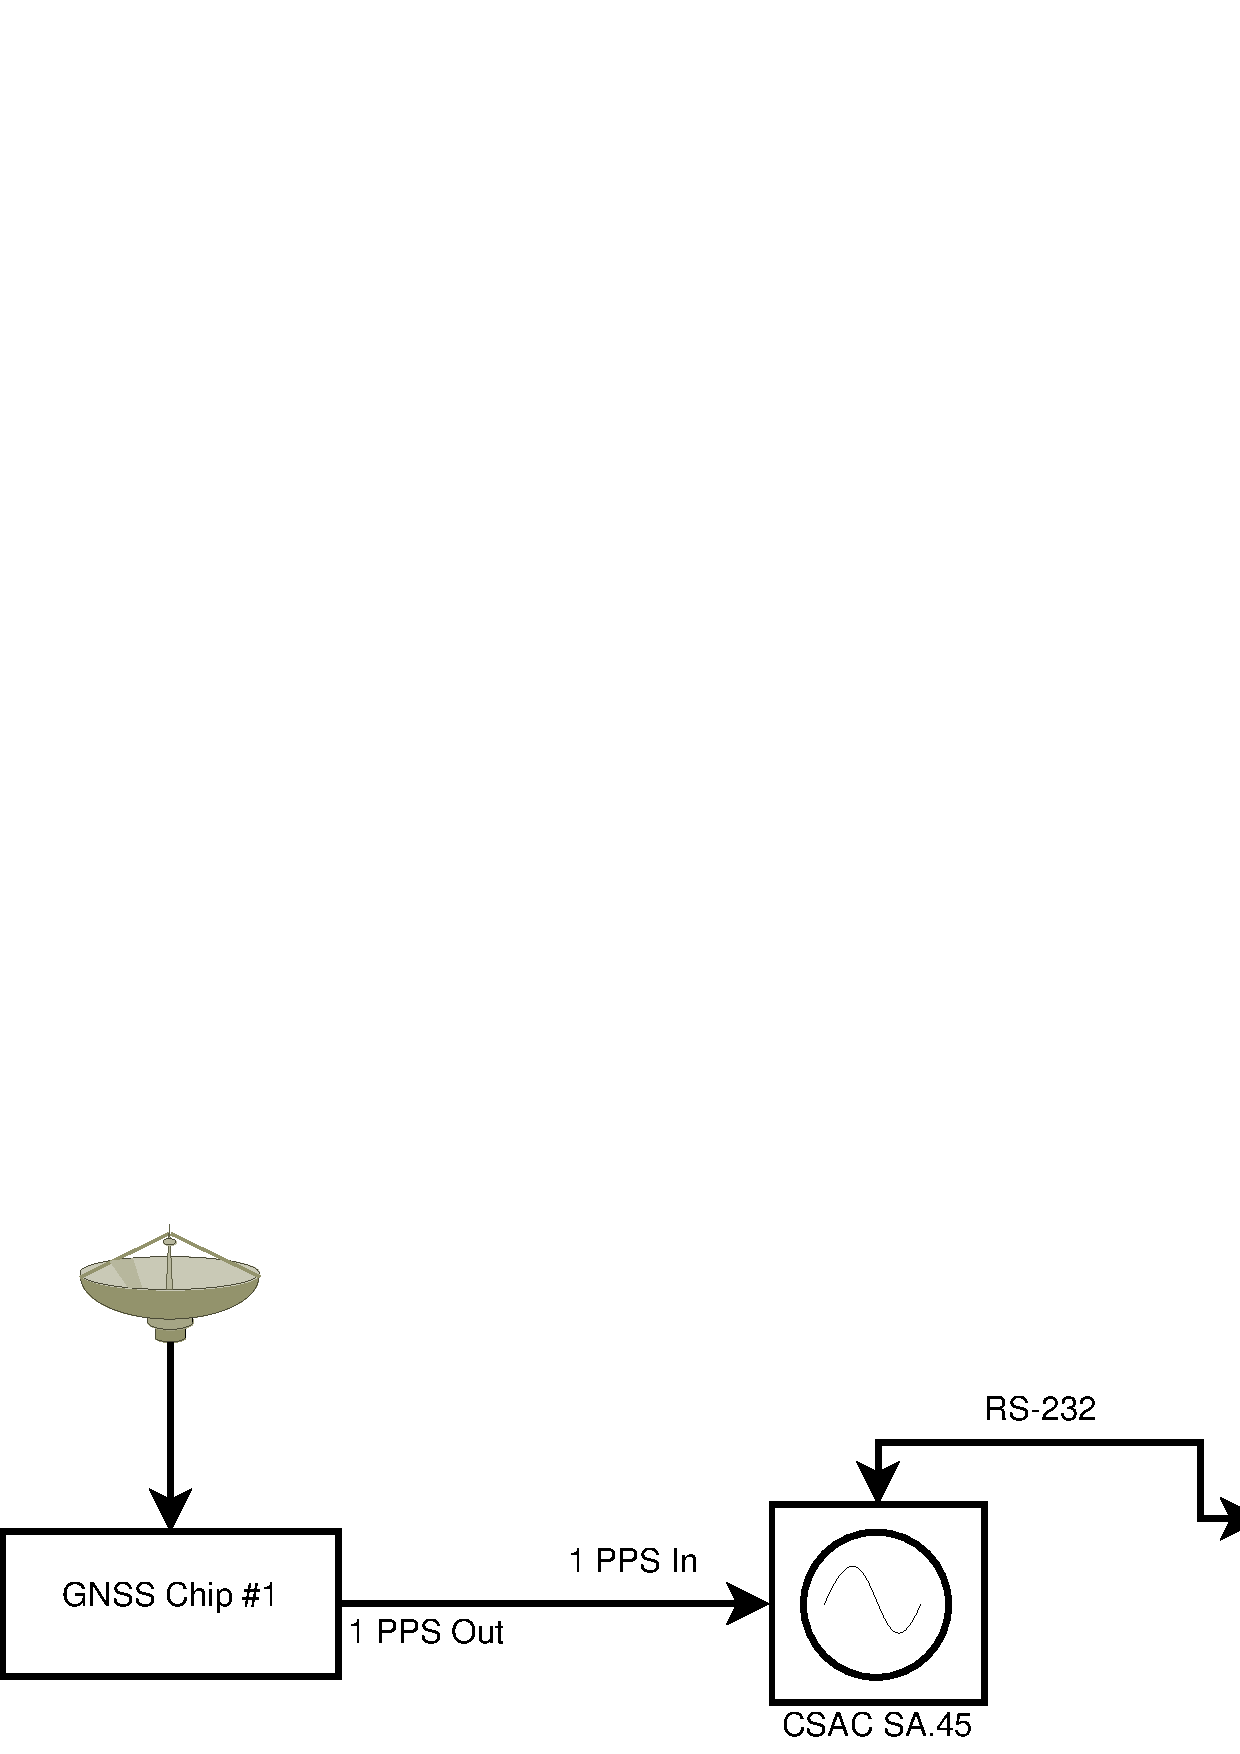
\includegraphics[scale=0.4]{csac_serial.pdf}
   \caption[Block diagram showing the CSAC connected to a PC]{Block diagram showing the CSAC connected to a PC}
   \label{csac_filter}
\end{figure}
The SA.45 CSAC includes a serial interface that enables communication with a PC by using a COM port. As mentioned earlier, our approach relies heavily on the ability to communicate with the CSAC.
Information can be queried by sending commands to the CSAC. These commands are explained in table \ref{CSAC_COMMANDS}. 
\begin{table}[]
\centering
\caption{Commands for the SA.45 CSAC}
\label{CSAC_COMMANDS}
\begin{tabular}{|l|l|l|}
\hline
Shortcut          & Description                                        & Command                       \\ \hline
6                 & Return telemetry headers as comma-delimited string & !6{[}CRLF{]}                  \\ \hline
\textasciicircum  & Return telemetry as comma-delimited string         & !\textasciicircum  {[}CRLF{]} \\ \hline
F                 & Adjust frequency                                   & !F?{[}CRLF{]}                 \\ \hline
M                 & Set operating mode register bits                   & !M?{[}CRLF{]}                 \\ \hline
S                 & Sync CSAC 1 PPS to external 1 PPS                  & !S{[}CRLF{]}                  \\ \hline
D                 & Set 1 PPS disciplining time constant               & !D?{[}CRLF{]}                 \\ \hline
U                 & Set ultra-low power mode parameters                & !U?{[}CRLF{]}                 \\ \hline
T                 & Set/report time-of-day                             & !T?{[}CRLF{]}                 \\ \hline
\end{tabular}
\caption*{Source: \cite{CSAC_USERGUIDE}}
\end{table}
In this document, the word \textit{telemetry} gets mentioned quite often in context with the CSAC. Telemetry can be obtained by querying the CSAC. The telemetry is a string containing a plethora of information, but we are mainly interested in the following values:
\begin{itemize}
  \item{Phase, the difference between the CSAC and the external signal signal at 1PPS in.}
  \item{DiscOK, the discipline status.}
  \item{Steer, the frequency adjust.}
\end{itemize}
The SA.45 uses a high-resolution phase meter to improve synchronization and to calibrate the frequency of the CSAC. The phase meter measures the difference in time between the internal PPS 1 PPS signal and the external reference, in our case, a GNSS receiver. This difference is the \textit{phase} value. The CSAC uses the phase value and steering algorithms to adjust the frequency of CSAC physics package thus simultaneously steering both the phase and frequency to that of the external reference. This is called \textit{disciplining} and is how the \textit{steer} value is computed. The last value, \textit{DiscOK} is simply the status of the 1 PPS disciplining routine. \cite{CSAC_USERGUIDE} (EXPLAIN THIS IN DETAIL). 

\section{Detection algorithms: Filters}
\subsection{Data acquisition}\label{data_aquisition}
In order to create an accurate clock-model of the CSAC, it was necessary to log data from it while it was running in a disciplined mode. In the disciplined mode, the CSAC will correct it's frequency based on either a 1 PPS (Pulse per second) signal or a 10 MHz signal. A similar approach was used in order to collect GPS data. Data from two u-blox NEO-M8T was gathered over the same time period as the data gathered from the CSAC. By gathering the data over the same period, it was possible to detect any correlation between the time solved by the GPS receivers and any frequency adjustments done by the CSAC. It also provided valuable data that could be used to tune the spoofing detection algorithms in the CSAC SMACC. The data gathering was done by simple Python scripts (\ref{CL} and \ref{GL}) running on a computer connected to the receivers and the CSAC (\ref{CLS})

\subsubsection{Clock Model (CM) based filter}\label{cmbf}
Write about clock model and the filters

\subsubsection{Known vs Reported location (KRL) filter}\label{kvsrlf}
As discussed during the introduction (\ref{cspakp}), an easy way to detect spoofing, is to check the GNSS receivers solved position against the known position of the receiver. The detection techniques efficiency also increases as more receivers are added to the detection setup. This is because it is hard to spoof a GNSS receiver without also spoofing it's neighbor. By accidentally spoofing the neighbor, the two GNSS receivers would solved the same position and position (depending on the spoofing technique), thus giving away the attempt. By configuring the Sensor Server with the location of the different Sensors, the server can act if Sensor reports an abnormal solved position. The filter is triggered when either latitude, longitude, altitude or speed is bigger or lower than the reference value minus or plus a deviation. Listing (\ref{ref_dev_filter_latitude}) shows an edited sample of code taken from \texttt{filters.c}. The code in the sample is part of the algorithm used to check whether or not the latitude part of the GNSS receivers solved position is within "safe" (not spoofed) range.
\begin{code}
  \caption{Sample of code taken from \texttt{filters.c} line 66. The code has been edited for clarity.}
    \begin{minted}
    [
      fontsize=\footnotesize,
      fontfamily=tt,
      linenos=true
    ]
    {c}
        if(latitude_current > latitude_reference + latitude_deviation) {
            moved = 1;
            lat_disturbed = HIGH;
        } else if(latitude_current < latitude_ref - latitude_dev) {
            moved = 1;
            latitude_disturbed = LOW;
        } else {
            latitude_disturbed = SAFE;
        }
    \end{minted}
    \label{ref_dev_filter_latitude}
\end{code}

\section{The Sensor Server}
In the following section, the architecture and inner workings, data structures and key components of the Sensor Server will be explained. 
The Server core(\ref{server_core}) consists of the source code in \texttt{sensor\_server.c}. The Parser and Handler spans over texttt{session.c} and texttt{actions.c}.

\subsection{Server core}\label{server_core}
\begin{figure}
\centering
  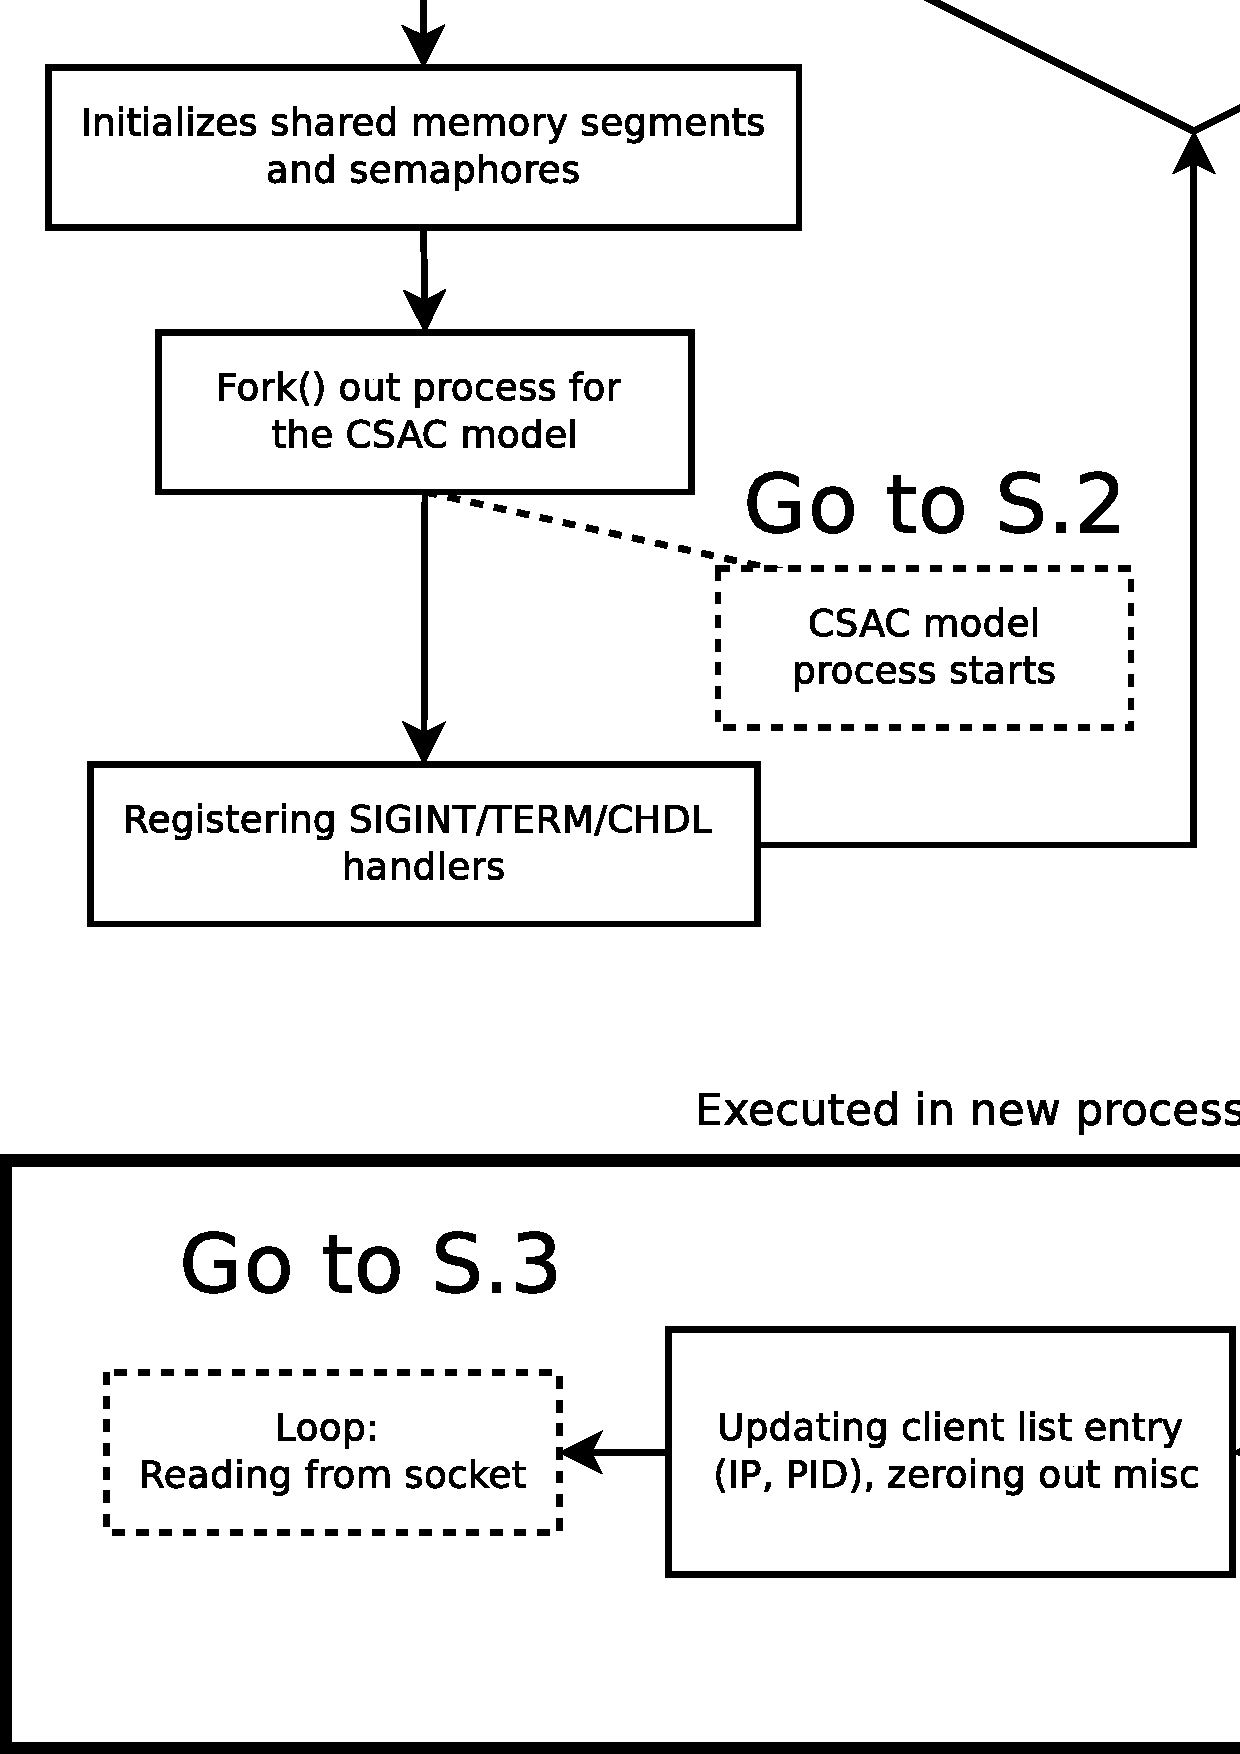
\includegraphics[scale=0.3]{server_core.pdf}
   \caption[Socket Server Core execution flow block diagram]{The block diagram shows an abstracted view of the Sensor Servers Core.}
   \label{server_core}
\end{figure}
The "Server core" is the main process and the parent of every process created during the life of the Sensor Server. It spawns the process maintaining the CSAC model as well as new processes for every client that connects. Figure \ref{server_core} is a block diagram of the Server core. 

\begin{itemize} % Sources needed here?
  \item The Server software takes one parameter to start, the port. If the parameter are missing or the parameter is illegal, a string containing usage information is printed and the program exits. Because the Server is responsible for the communication with the CSAC, it needs to be run as root or with \texttt{sudo} in order to open the serial interface to the CSAC.
  \item The configuration is initialized on loaded (see (\ref{config_loader}) for more). If the configuration fails to load, the Server prints and error message and exits.
  \item The \texttt{client\_list}, a linked list(\ref{linked_list}) containing all the clients, is initialized.
  \item Shared memory segments (\ref{shared_mem_sem}) and semaphores are initialized and allocated. If this fails, the Server prints an error message and exits.
  \item The process responsible for maintaining the CSAC model, communication with CSAC and filters associated with the CSAC, is forked out. If the fork fails, the server prints an error message and exits.
  \item Handler for SIGINT (interrupt) SIGTERM (terminate) and SIGCHLD (child process is interrupted or terminated) is registered.
  \begin{itemize}
      \item When a process exits, a SIGCHLD signal is sent to the parent. When a client disconnects from the server, the process that handled the client exits. Ideally, the client disconnects from the server by sending a protocol compliant "disconnect request". This wau, the server can handle the disconnect in a controlled manner and update its client list when the client disconnects. However, this is not always the case and if the client disconnects abruptly and without a warning, the server still needs to handle it. Therefore, when a SIGCHLD signal is received, the server iterates through its client list and finds the client who's PID matches the sender of the signal and removes it from the list. In figure \ref{server_core} this routine is the part in the red dotted box. 
  \end{itemize}
  \item The socket is initializes (\ref{sockets}) and marked for listening.
  \item A loop is entered. The loop breaks when \texttt{volatile sig\_atomic\_t done} equals 0. If the loop is broken, the semaphores are destroyed and all allocated memory is freed, the servers socket file descriptor is closed and the Server exits.
  \item When a client connects, the server checks if the maximum number of clients has been reached. If this number has been reached, an error message is written back to the client and the clients socket file descriptor is closed. If the maximum number of clients has not yet been reached, the client list gets updated and a fork is performed.
  The parent process then resumes the loop. 
  \item The process that just forked out for the new connection closes the server socket file descriptor it inherited from its parent. 
  \item The new process then updates its client table entry (\ref{client_table_entry}) and proceeds to the listening loop (\ref{parser_and_handler}).
\end{itemize}

\subsection{CSAC model}
\begin{figure}
\centering
  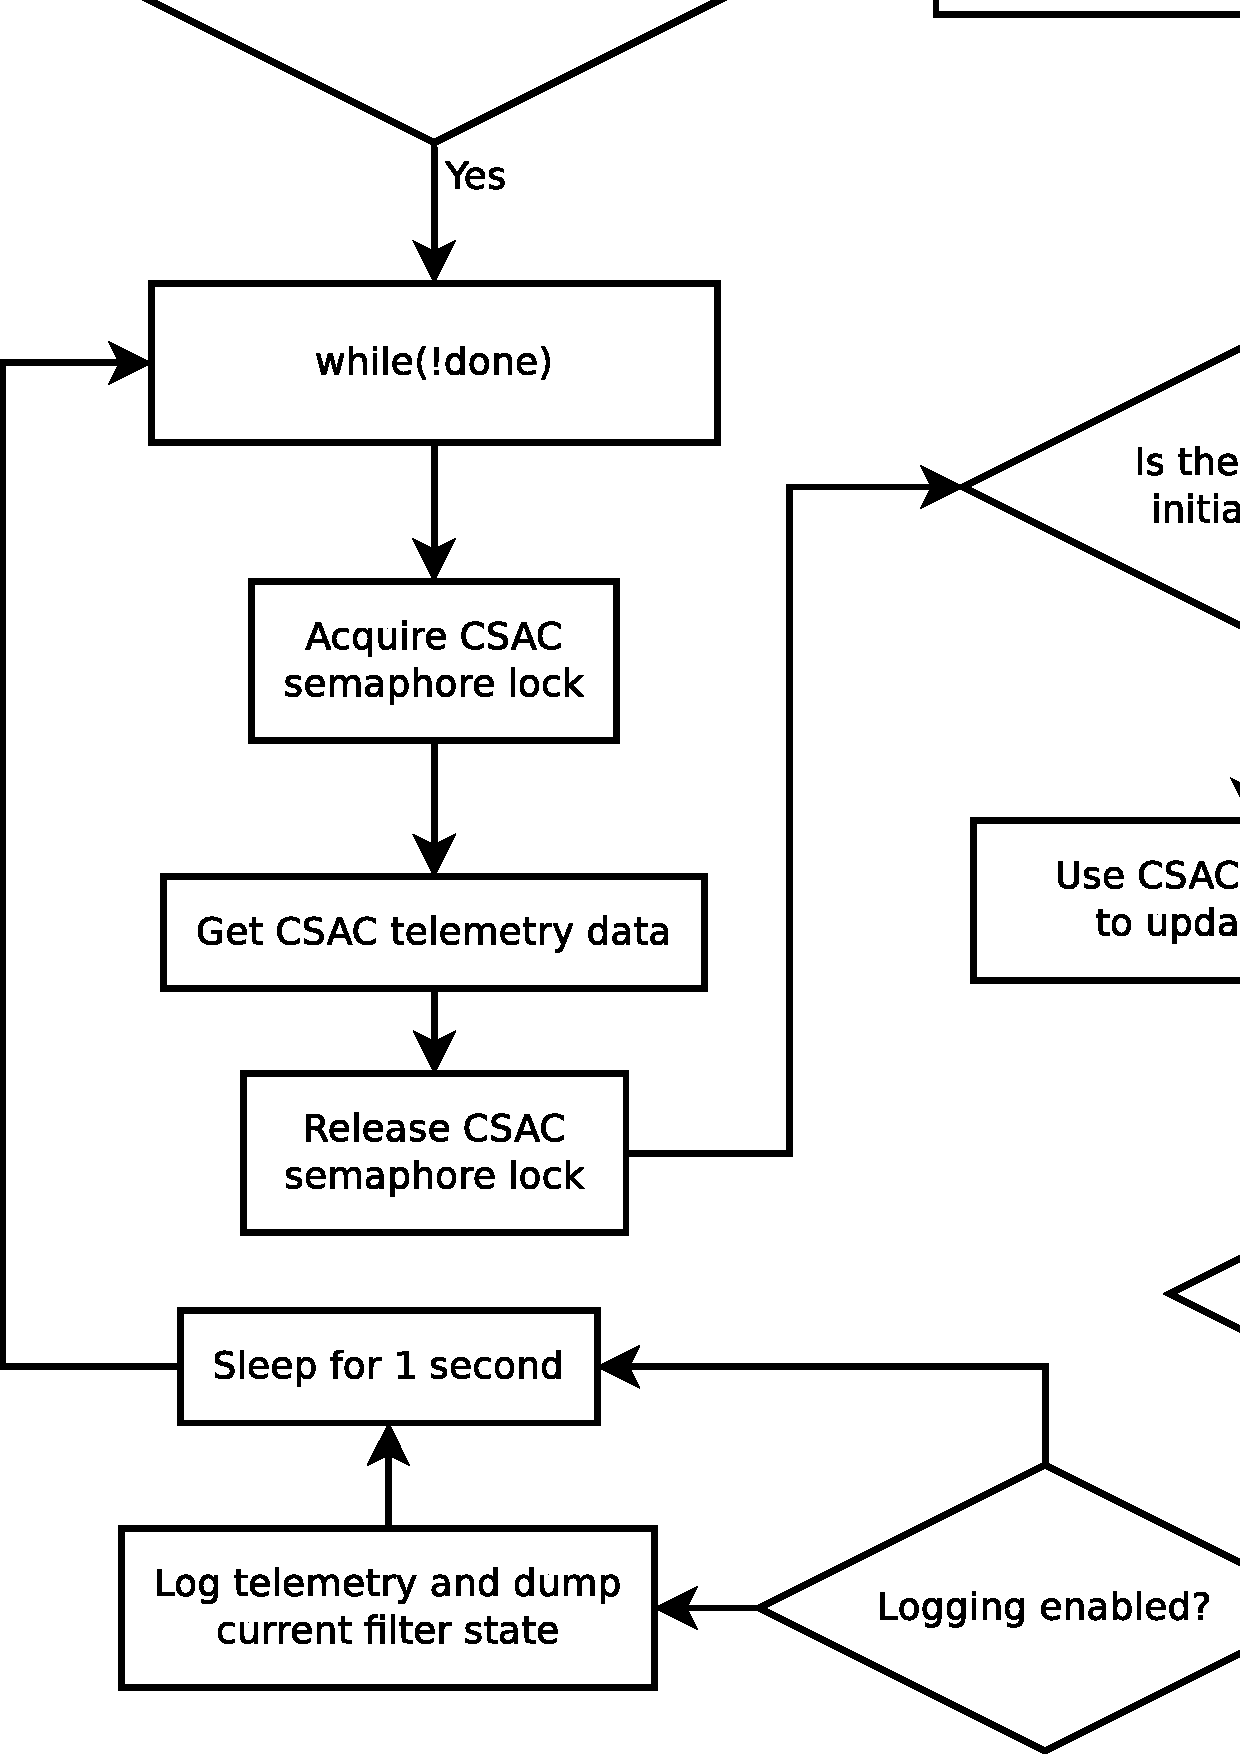
\includegraphics[angle=90, scale=0.30]{csac_filter_model.pdf}
   \caption[CSAC model execution flow block diagram]{Block diagram showing the flow of execution in the CSAC model}
   \label{csac_filter}
\end{figure}
The CSAC model is a model of the CSAC. In short, it is used to determine the validity of the disciplining the CSAC is subjected to. As discussed earlier, the CSAC is disciplined by a 1 PPS signal generated by a GNSS receiver. If that GNSS receiver is spoofed, the model can be used to detect the spoofing by calculating the predicted steer values and comparing them with the current ones being applied by the CSACs internal steer algorithms. Conceptually, the CSAC model and the filter that uses the model, is to separate tasks. In practice however, they are intertwined. 
\begin{itemize}
  \item The configuration for the model is loaded. The configuration includes values defining the accepted limits for steering and phase difference. It also includes values that can be used to restore the state of the model thus reducing the time it takes for the model to become suitable for the use as a reference. If the loading of the configuration fails, and error message is printed, the \texttt{volatile sig\_atomic\_t done} is set to 1 and the process exits.
  \item A loop is entered. The loop breaks when \texttt{volatile sig\_atomic\_t done} equals 0. 
  \item The CSAC lock(\ref{shared_mem_sem}) is acquired and once the telemetry is queried from the CSAC, it is released again.
  \item If the model is not initialized, telemetry data is used to initialize it. If "state-restoring" values are present in the earlier loaded configuration, these will now also be used to initialize the model even further.
  \item If the model is already initialized, the telemetry received from the CSAC is used to update the model. 
  \item A check is done to see how long the model has been running and "fed" with data. The model needs to gather data over time in order to become accurate enough to be used as a reference. The time needed is configurable, but typically, 2 days are enough. 
  \item If the model has been running for long enough, it can be used as a reference in a filter and detect spoofing attempts. Either way, the telemetry is logged and the current state is dumped to file. The state dump is actually done every time the filter is updated and overwrites the previous state file. This is not a bug, but meant as a "nice-to-have" mechanism in case a user of the system forgets to note down the state of filter and planned to use the data later during initializing. 
  \item If the model is old enough to be used for filtering (spoofing detection), the absolute value of current steer as read from telemetry is compared with the predicted steer value derived from the model. If it is bigger, the alarm is logged, the CSAC is taken out of disciplining mode and steer value from the model is used.
\end{itemize}

\subsubsection{Notes}


\subsection{Parser and Handler}\label{parser_and_handler}
\begin{figure}
\centering
  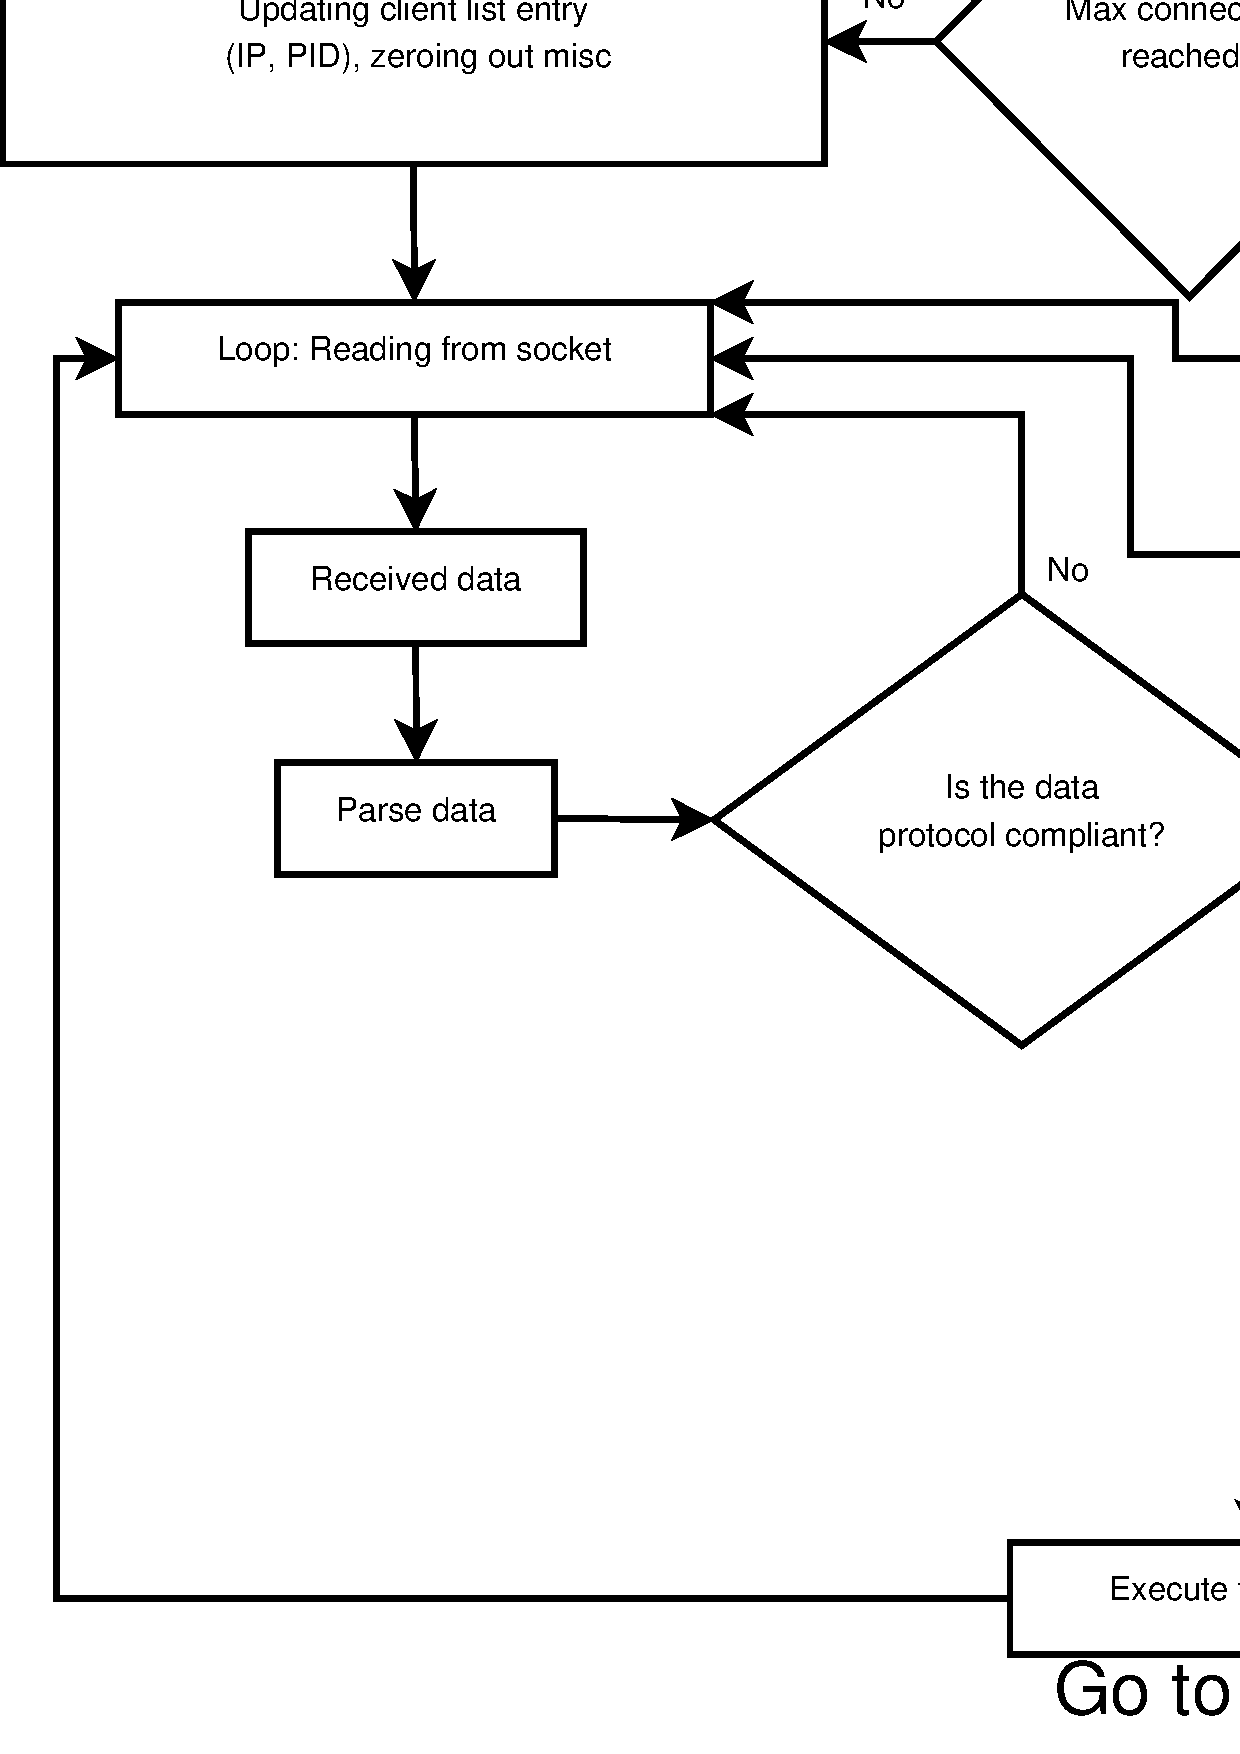
\includegraphics[angle=90,scale=0.3]{server_flow.pdf}
   \caption[Socket Server execution flow block diagram]{The block diagram shows an abstracted view of execution after a client has connected to the server and a \texttt{fork()} has been performed.}
   \label{server_flow}
\end{figure}
\begin{figure}
\centering
  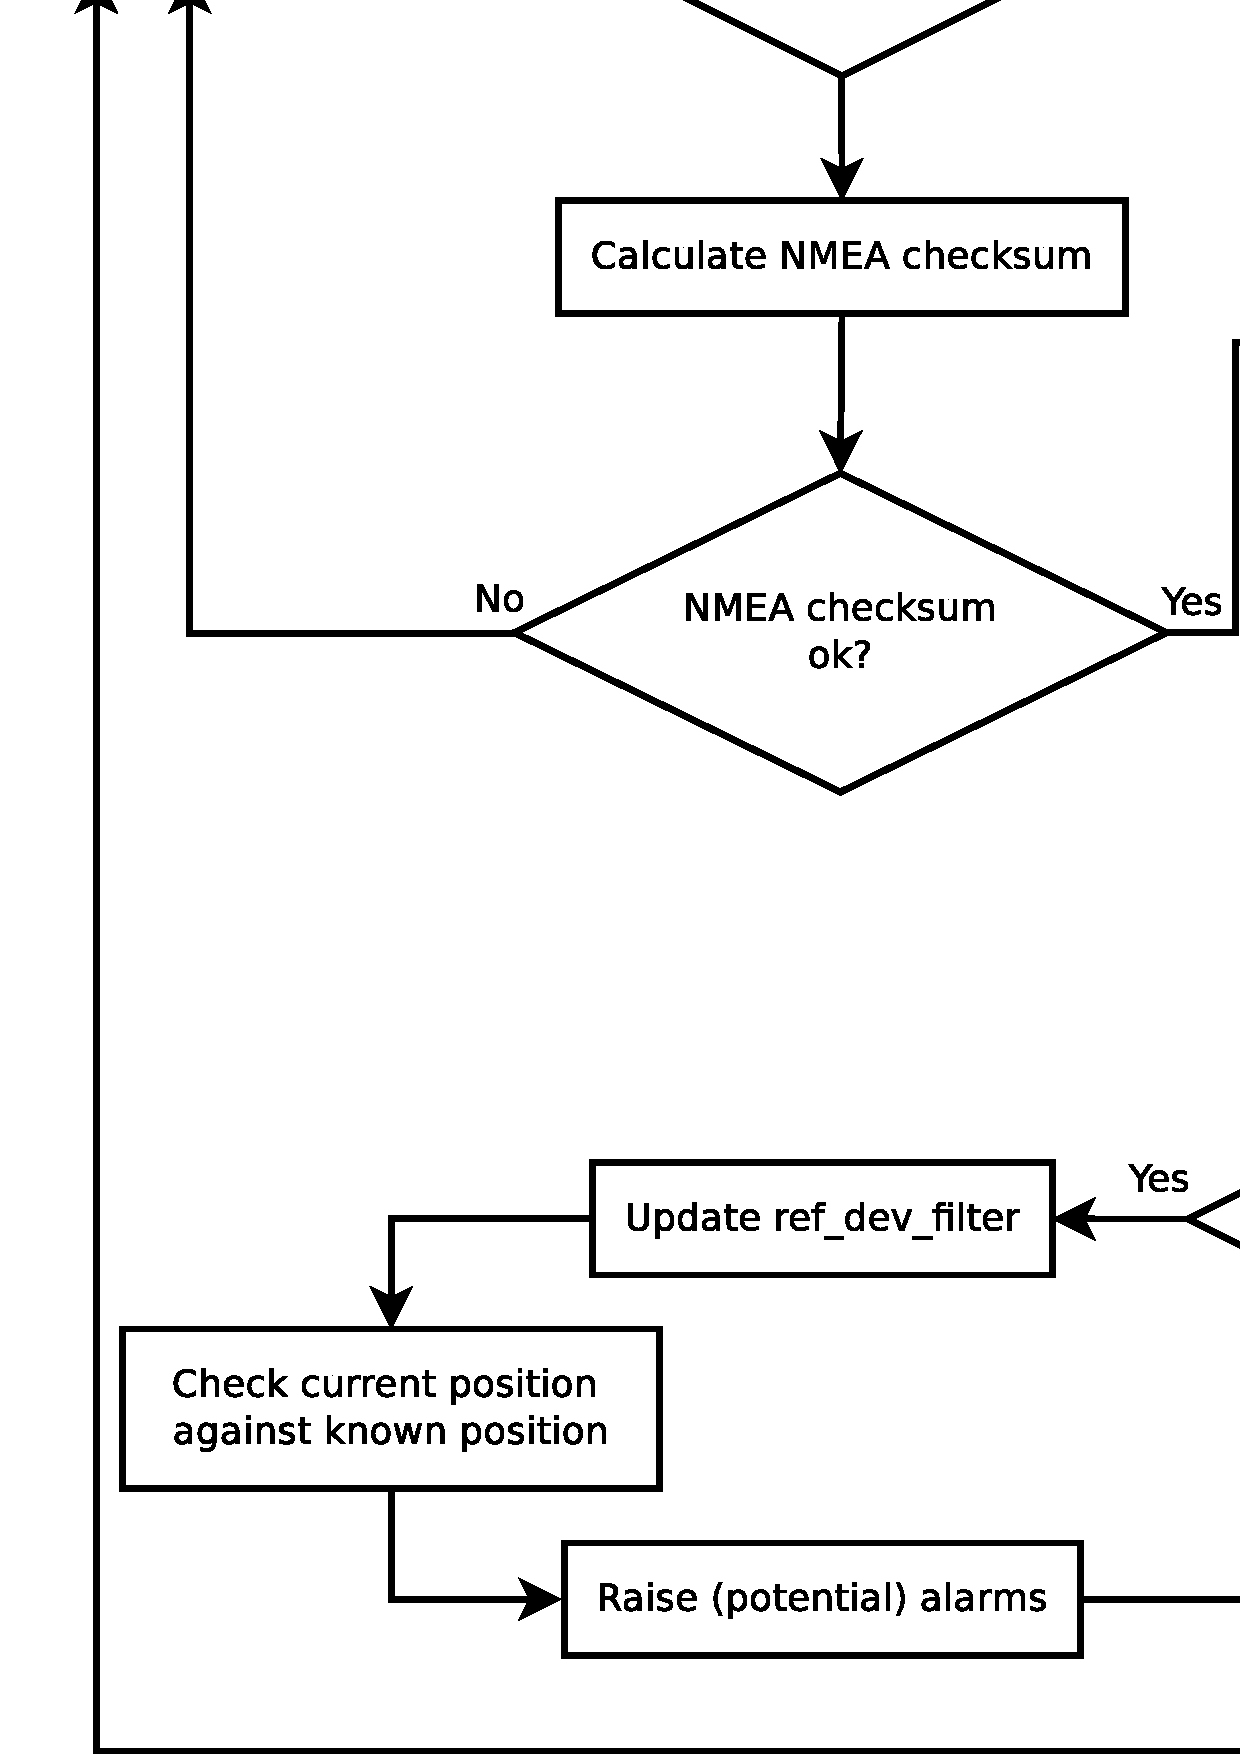
\includegraphics[scale=0.40]{actions_core.pdf}
   \caption[Socket Server execution flow block diagram]{The block diagrams shows and abstracted view of the execution after data has been received from a client.}
   \label{actions_core}
\end{figure}
The parser and handler are responsible for parsing data received from a client and making sure every request is protocol compliant. Once the goal of the request has been established, the request is executed. Figure \ref{server_flow} and \ref{actions_core} are block diagrams showing the execution flow for this part of the server.  
\begin{itemize}
  \item A loop is entered. The loop is broken when \texttt{volatile sig\_atomic\_t done}\label{atomic_done} equals 0. This is the same variable that is used in the Server core \ref{server_core} loop and for a good reason: If the server exits, then the its children should too. 
  \item If reading from the socket fails, the client gets disconnected. If it is successful, the client table entry for the connected client is checked to see if the client has been marked to be kicked. If it is, it gets disconnected. 
  \item The data received from the client is parsed and checked against the protocol. If the request received from the client doesn't match any of the supported requests or commands, the request is ignored and the loop is entered again. 
  \item If the request received is valid, the clients ID is checked to determine whether or not it has identified itself. If the client has identified itself, the request gets carried out. 
  \item If the request received is to handle NMEA data, the checksum for that NMEA data is calculated. If the checksum check fails, the data is discarded. If it succeeds, the data is copied into \texttt{nmea\_container} struct (\ref{nmea_cont}) for easier handling.
  \item The client is marked as ready for processing and a ready check is commenced. The ready check is used to make sure that all the sensors have received NMEA data and are ready to have filters applied. Once the filters have been applied, the lock is released and normal execution resumes.
  \item If the clients ID is 0, it is considered unidentified and any other requests but to identify itself, is ignored.
  \item If the client is attempting to identify itself, the ID it attempts to use is checked against the rest of the connected clients. If the ID is already taken and the client attempted to assume the role of a Sensor, the client will get disconnected. If it attempted to assume the role of a Monitor, it will simply be notified that the chosen ID is taken and the request will be ignored. The reason why a Sensor would get disconnected and a monitor would not, is simple: When connecting the Sensor to the server, it should not be any doubt whether or not it has been accepted. If something is wrong, it is better that a user of the system has to deal with it there and then and configure the Sensor correct rather than allowing the user to do mistakes which reduces the efficiency of the system. 
  \item If the attempted ID is available, the client table entry for the client is updated with the requested ID and the server will attempt to load KRL (\ref{kvsrlf}) filter data into the clients KRL filter struct. The server will attempt to load the data from a file named \texttt{krl\_data\_sensor<ID>}. If the load fails, the client will be disconnected. It is after all useless without its reference position data.
\end{itemize}

\subsection{Data structures}
In the C programming language, a "struct" is a complex data type that defines a list of variables to be placed under the structs given name in a block of memory. This makes it possible for multiple variables to be accessed via a single pointer. Before delving deeper into the code base of the sensor server, some crucial and often used structs will be explained in this section.

\subsubsection{client\_table\_entry}\label{client_table_entry}
The client\_table\_entry struct is what the name suggests, it's an entry in a list of clients. Every client connected to the server, no matter the purpose, has an entry in the client list. Listing \ref{struct_client_table} shows the complete struct. 

\begin{code}
  \caption{Sample of code taken from \texttt{sensor\_server\_common.h} line 99}
    \begin{minted}
    [
    fontsize=\footnotesize,
    fontfamily=tt,
    linenos=true
    ]
    {c}
    struct client_table_entry {
        struct list_head list; 
        struct transmission_s transmission; 
        struct timeval heartbeat_timeout; 
        struct command_code cm;   
        struct nmea_container nmea;    
        pid_t pid;  
        time_t timestamp;  
        int client_id; 
        int client_type;    
        int ready;  
        int marked_for_kick; 
        char ip[INET_ADDRSTRLEN];
        struct filters fs;
    };
    \end{minted}
    \label{struct_client_table}
\end{code}
Beginning from the top:
\begin{itemize}
  \item \texttt{list\_head list} is a pointer to a 
\end{itemize}

\subsubsection{server\_data}
\begin{code}
  \caption{Sample of code taken from \texttt{sensor\_server\_common.h} line 116}
    \begin{minted}
    [
    fontsize=\footnotesize,
    fontfamily=tt,
    linenos=true
    ]
    {c}
    struct server_data {
        int number_of_clients; 
        int number_of_sensors;  
        time_t started;    
        pid_t pid;             
        char version[4]; 
    \end{minted}
  \label{server_data}
\end{code}
The \texttt{server\_data} struct contains information about the server. Some of the of information like the PID, version, and when the server was started, is just information about the server itself. The number of clients and sensors on the other hand, is used to make sure that the server does not allow more connections than it can handle.

\subsubsection{server\_synchro}
\begin{code}
  \caption{Sample of code taken from \texttt{sensor\_server\_common.h} line 125}
    \begin{minted}
    [
    fontsize=\footnotesize,
    fontfamily=tt,
    linenos=true
    ]
    {c}
    struct server_synchro {
        sem_t ready_sem;
        sem_t csac_sem;
        sem_t client_list_sem;
    };
    \end{minted}
  \label{server_synchro}
\end{code}
The \texttt{server\_synchro} structs member are semaphores (\ref{shared_mem_sem}) that the server and its children processes uses to protect atomic access to shared resources. The \texttt{csac\_sem} is used to control serial access to the CSAC, making sure that only one request is sent to CSAC at a time. The \texttt{client\_list\_sem} is used by functions manipulating and reading the client list structure, and the \texttt{ready\_sem} is only used when the server has received NMEA data and a ready check has been initiated (\ref{nmea_ready}).

\subsubsection{command\_code}
\begin{code}
  \caption{Sample of code taken from \texttt{sensor\_server\_common.h} line 34}
    \begin{minted}
    [
    fontsize=\footnotesize,
    fontfamily=tt,
    linenos=true
    ]
    {c}
    struct command_code {
        int code;
        char parameter[MAX_PARAMETER_SIZE];
        int id_parameter;
    };
    \end{minted}
  \label{command_code}
\end{code}

\subsubsection{NMEA container}\label{nmea_cont}
\begin{code}
  \caption{Sample of code taken from \texttt{nmea.h} line 21}
    \begin{minted}
    [
    fontsize=\footnotesize,
    fontfamily=tt,
    linenos=true
    ]
    {c}
    struct nmea_container {
        /* Raw data */
        char raw_gga[SENTENCE_LENGTH];
        char raw_rmc[SENTENCE_LENGTH];

        /* Latitude */
        double lat_current;
        double lat_average;
        double lat_avg_diff;
        double lat_total;
        int lat_disturbed;

        /* Longitude */
        double lon_current;
        double lon_average;
        double lon_avg_diff;
        double lon_total;
        int lon_disturbed;

        /* Altitude */
        double alt_current;
        double alt_average;
        double alt_avg_diff;
        double alt_total;
        int alt_disturbed;

        /* Speed */
        double speed_current;
        double speed_average;
        double speed_avg_diff;
        double speed_total;
        int speed_disturbed;

        /* CHECKSUM */
        int checksum_passed;

        /* COUNTER FOR AVERAGE */
        int n_samples;
    };
    \end{minted}
    \label{nmea_container}
\end{code}
The \texttt{nmea\_container} struct is a member

\newpage
\section{Interfacing}\label{interface}
As mentioned earlier (\ref{roles}), a client can assume the role of both a Monitor and a Sensor. The Sensor Server does not differentiate between the two roles other than when it routinely checks the status of its filters. This means that one could connect to the server using the Sensor Client software as a Monitor by configuring the Sensor Client software to use a negative integer as ID. At this point, this kind of functionality is not very useful as there is currently no way to change the ID of a client unless the client explicitly issues the command to do so, but it opens for the possibility to interface with the server. One way to interface with the Sensor Server is to connect to it using Telnet:

\begin{lstlisting}
user@machine:/$ telnet 10.1.0.46 10001
Trying 10.1.0.46...
Connected to 10.1.0.46.
Escape character is '^]'.
ID -3
OK!

>
\end{lstlisting}
It is also possible to assume the role of a Sensor by connecting to the server via telnet. This can be used to debug or troubleshoot the Sensor Server by manually feeding it NMEA data. The only requirement is that the communication is Sensor Server protocol compliant:

\begin{lstlisting}
user@machine:/$ telnet 10.1.0.46 10001
Trying 10.1.0.46...
Connected to 10.1.0.46.
Escape character is '^]'.
ID 2
OK!

NMEA<GNRMC part of NMEA><GNGGA part of NMEA>
OK!
\end{lstlisting}
Another possibility is off course to write scripts that communicates with the Sensor Server. An example script can be found in the appendix (\ref{script_example}).

\begin{table}
	\caption{Sensor Server available commands}
	\label{commands}
	\begin{tabularx}{\textwidth}{|l|l|l|X|}
	  \multicolumn{1}{l}{Command} & \multicolumn{1}{l}{Short} & \multicolumn{1}{l}{Parameter} & \multicolumn{1}{l}{Description}                                                                \\ \hline
	  HELP                        & ?                         & NONE                          & Prints this table                                                                              \\ \hline
	  IDENTIFY                    & ID                        & ID                            & Clients ID is set to PARAM                                                                     \\ \hline
	  DISCONNECT                  & EXIT                      & NONE                          & Disconnect from the server                                                                     \\ \hline
	  PRINTCLIENTS                & PC                        & NONE                          & Prints an overview of connected clients                                                        \\ \hline
	  PRINTSERVER                 & PS                        & NONE                          & Prints server state and config                                                                 \\ \hline
	  PRINTTIME                   &                           & ID                            & Prints time solved from GNSS data received from Sensor \textless ID\textgreater                 \\ \hline
	  PRINTAVGDIFF                & PAD                       & NONE                          & Prints the difference between current solved position and the average reported for all Sensors \\ \hline
	  PRINTLOC                    & PL                        & ID                            & Print solved position for Sensor \textless ID\textgreater                                       \\ \hline
	  LISTDATA                    & LSD                       & NONE                          & List all dump files stored by the server                                                       \\ \hline
	  DUMPDATA                    & DD                        & ID \& FILE                    & Dumps state of Sensor \textless ID\textgreater into a file named \textless FILE\textgreater      \\ \hline
	  LOADDATA                    & LD                        & ID \& FILE                    & Load state stored in file called \textless FILE\textgreater into Sensor \textless ID\textgreater \\ \hline
	  QUERYCSAC                   & QC                        & COMMAND                       & Queries the CSAC with COMMAND.                                                                 \\ \hline
	  LOADRFDATA                  & LRFD                      & ID                            & Load reference location data into Sensor \textless ID\textgreater                               \\ \hline
	  PRINTCFD                    & PFD                       & NONE                          & Prints CSAC filter data\\ \hline                                                                        
	  \end{tabularx}
\end{table}

\newpage
\section{The Sensor Client}\label{sensor_client}
The sensor client software is a simple program written in C99 whose only task is to relay information read from the GNSS receivers. Summed up shortly:
\begin{itemize}
  \item The client software takes two parameters to start, the servers IP and port. If parameters are missing, the program exits.
  \begin{itemize}
    \item Example: \texttt{./sensor\_client -p 10000 -i 192.168.1.5}
  \end{itemize}
  \item Initializes and loads configuration from configuration file. The configuration file includes path to the GNSS receiver, the sensors ID number and a binary value for whether or not logging of NMEA should be done as well as path to 
  the log file. If the loading of the configuration file fails, default values are used instead:
  \begin{itemize}
    \item The ID number is chosen at random but within legal limits.
    \item Logging is disabled.
    \item Maximum of server connection attempts are set to 10.
    \item Path to GNSS receiver is set to \texttt{/dev/ttyACM0}. This should be the path to the receiver unless another similar device is connected to the computer and given it is a Raspberry Pi running Raspbian.
  \end{itemize}
  \item Establishes communication with GNSS receiver, exits if it fails.
  \item Attempts to establish communication with the server, retries for a configurable amount of times at 1 second intervals.
  \item Identifies the client for the server according to protocol.
  \item Reads from the GNSS receiver, scans for lines starting with either \texttt{\$GNRMC} or \texttt{\$GNGGA}. When both lines are found, the data is stored in a buffer.
  \item Sends the GNSS data to the server according to protocol.
  \item Repeats.
\end{itemize}

\begin{figure}\label{client_call_graph}
\centering
  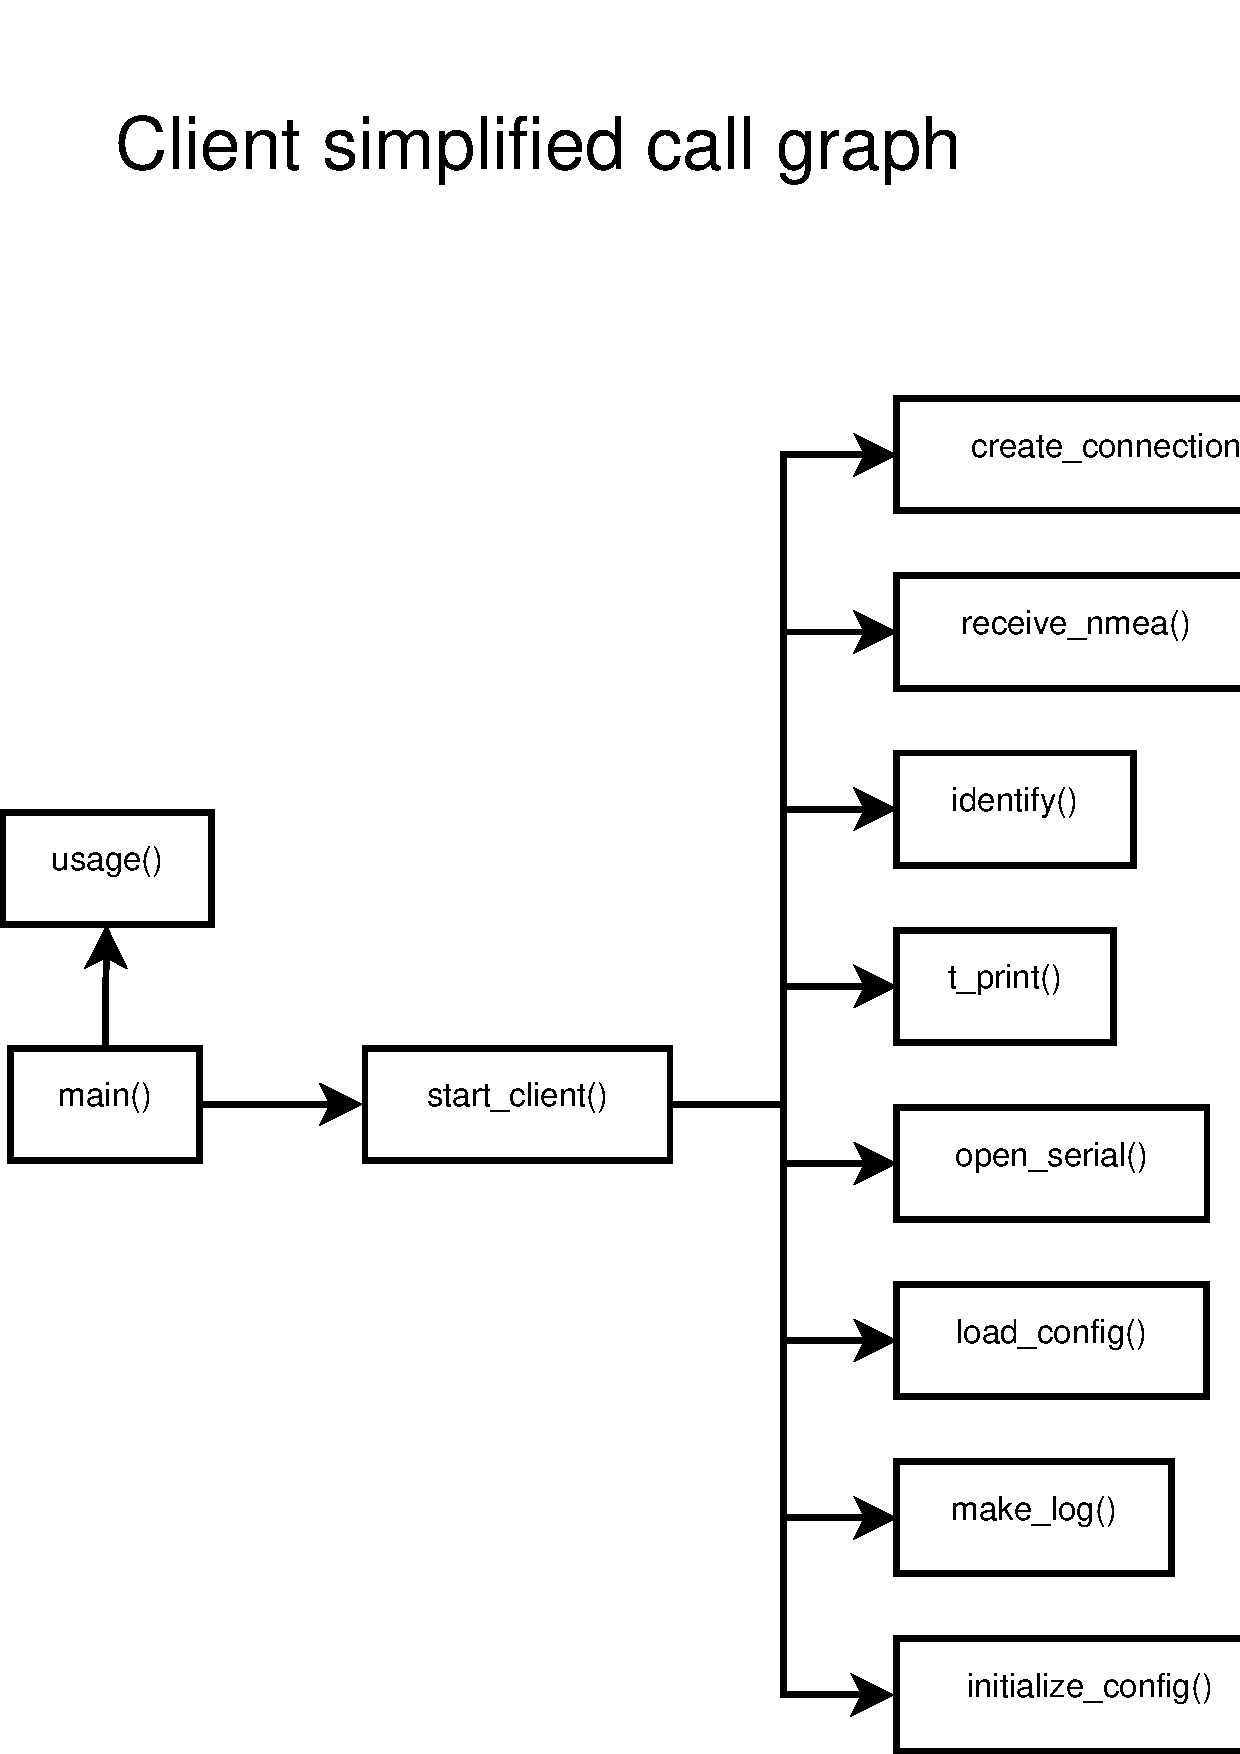
\includegraphics[scale=0.3]{client_call_graph.pdf}
   \caption[Sensor Client simplified call graph]{Simplified call graph for the Sensor Client.}
\end{figure}


\chapter{Testing}

\section{Spoofing simulation test}
When a GNSS receiver is spoofed, its solved position or time (or both) might change. The result depends on the technique used to spoof. By moving a GNSS receiver, one can simulate a spoofing attack since the location most certainly will change. It might also affect the time solved. (prat med Harald, dette er en problematisk forklaring). We also covered the antennas with aluminium foil to simulate a loss of signal. 

\subsection{Setup}
\begin{figure}
\centering
  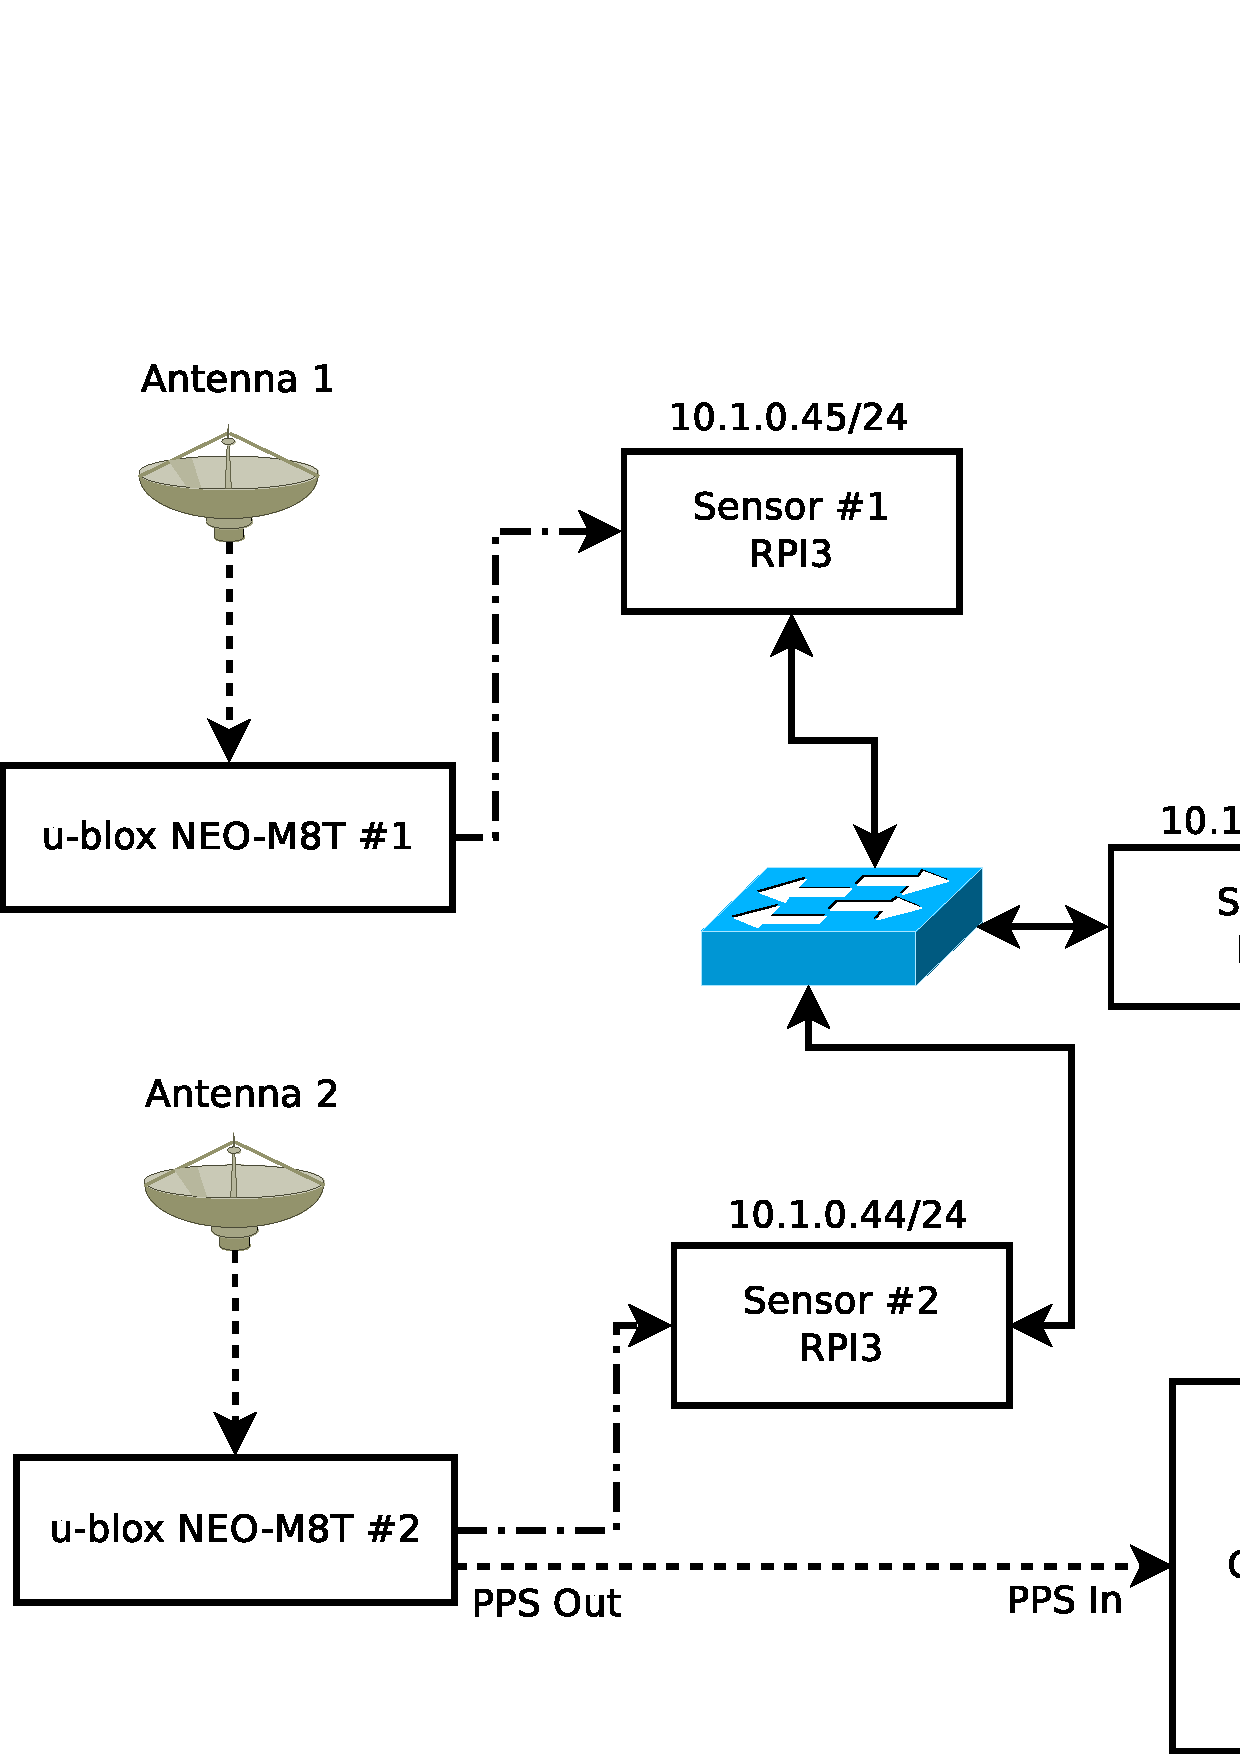
\includegraphics[scale=0.31]{server_layout.pdf}
   \caption[CSAC SMACC implementation block diagram]{A block diagram showing the tested implementation.}
   \label{ibd}
\end{figure}
Figure \ref{ibd} shows how the Server, Sensors and CSAC where physically set up. In order to assure good GNSS satellite geometry, the antennas where placed at a roof. Antenna 1 was placed at a railing about a 1 meter above the ground, antenna 2 was placed at ground level. Antenna 1 was connected to GNSS receiver 1 which in turn was connected to Sensor 1. It's the same deal with antenna 2 which was connected to GNSS receiver 2 which in turn was connected to Sensor 2. The distance between the two antennas was about 35 meters. The Sensors and the Server where connected to LAN through a Gigabit ethernet switch. The Server was configured to log telemetry received from the CSAC and the Clients where configured to log all NMEA data received from the GNSS receivers. The GNSS receiver connected to antenna South is used to supply the CSAC with a 1 PPS signal. Because the CSAC model needs live data over time to mature, the system was started Friday 7. October and the test was performed Monday 10. October.

\begin{figure}
\centering
  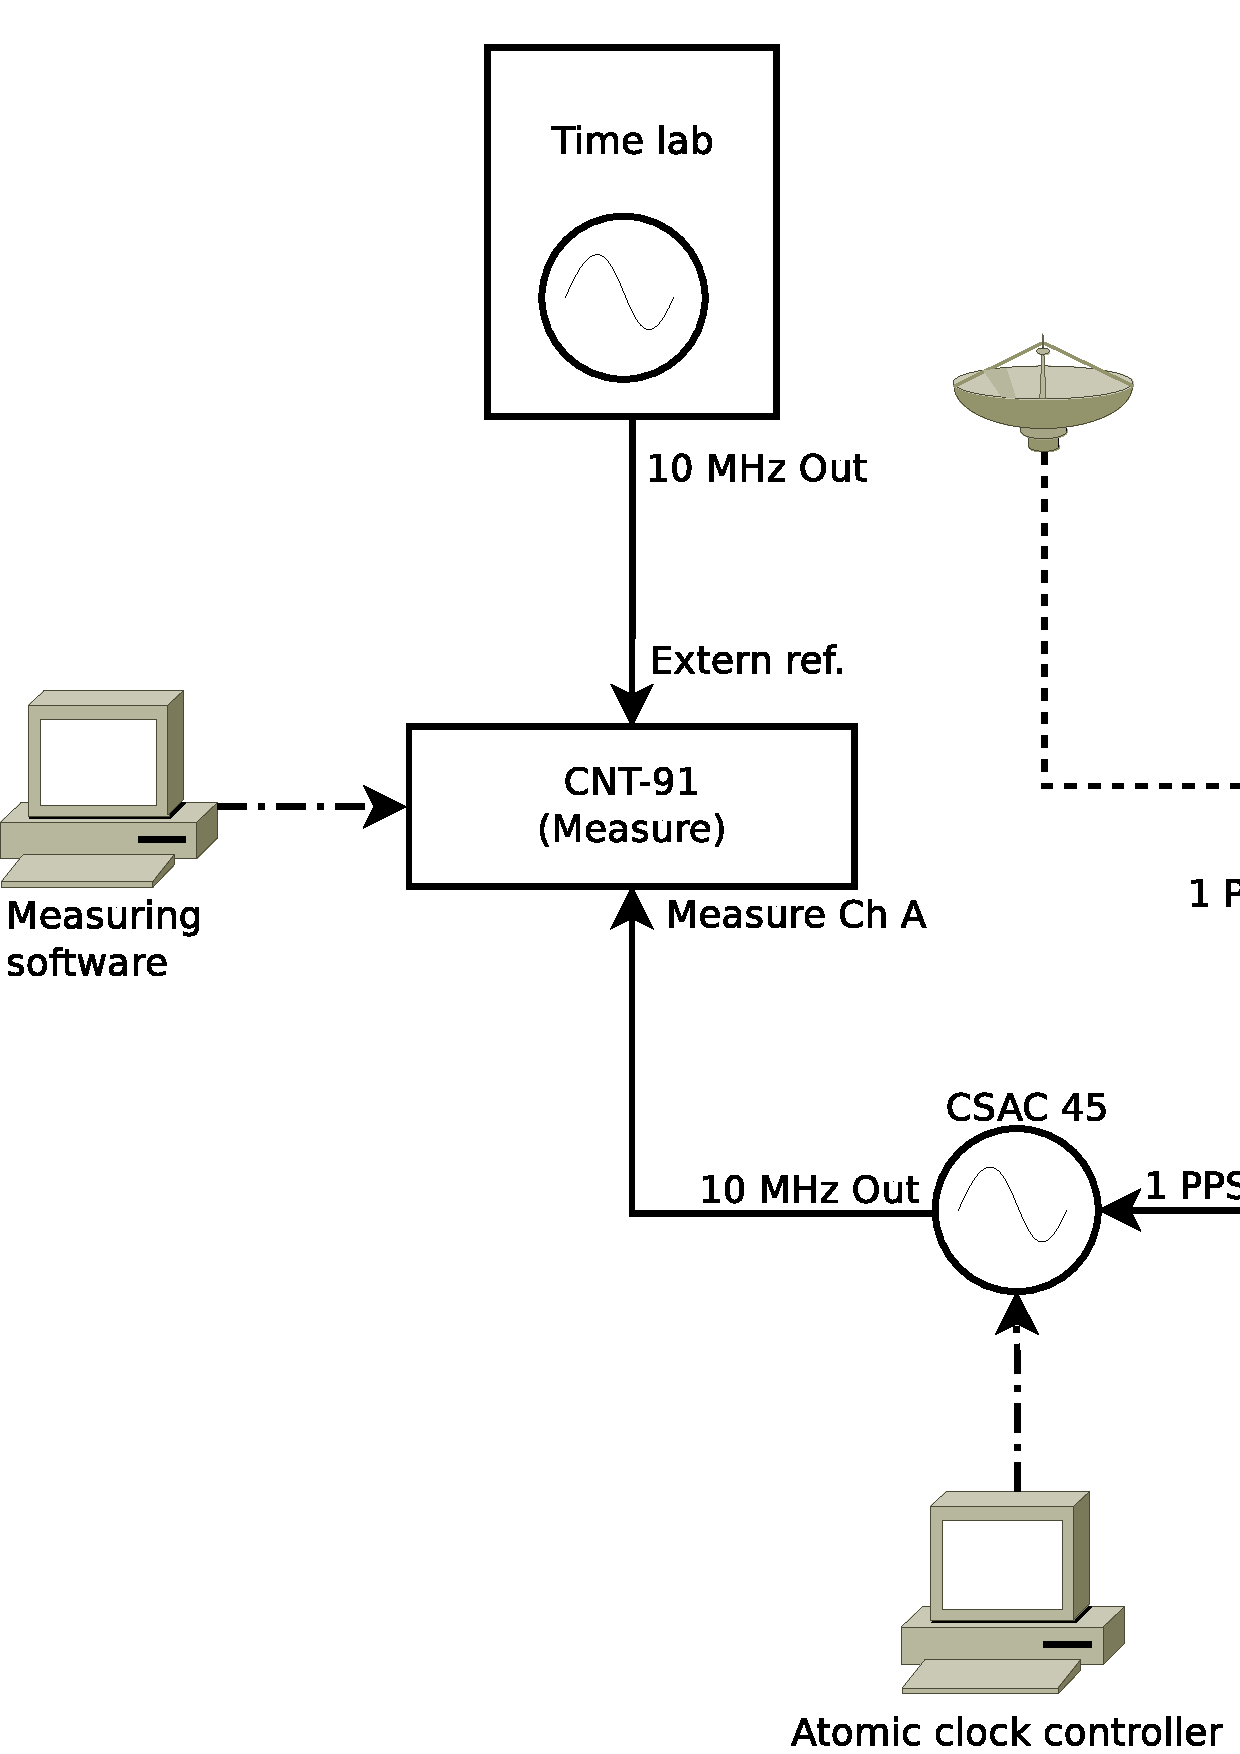
\includegraphics[scale=0.31]{measure_setup.pdf}
   \caption[Measurement setup]{Block diagram showing the setup of the measurement equipment}
   \label{msd}
\end{figure}
! DESCRIBE THE DETAILS OF THEM MEASUREMENT HERE !

\subsection{Goal of test}
The goal with this test was to use the CSAC SMACC to detect a simulated spoofing attack. By moving the antennas, the KRL filter(\ref{kvsrlf}) should be triggered as the solved longitude, altitude, latitude and speed should change. The CM might also trigger (men hvorfor?). The result would be observable by analyzing the log files produced by the Server and Clients.

\subsection{Description}\label{description}
The following is a step by step description of how the test was conducted. The time was obtained from a simple wristwatch, neither the resolution or accuracy was of any notable concern. The reason why the time is noted, is to make it easier to find any correlation between the steps taken and patterns found in the log files.

\begin{enumerate}
  \item Moved antenna 1 approximately 15 meters to the south (10:58).
  \item Moved antenna 1 back to original location (11:03).
  \item Moved antenna 2 approximately 15 meters to the north (11:07).
  \item Moved antenna 2 back to original location (11:12).
  \item Waved antenna 1 around horizontally in a half circle motion at an increasing tempo (11:14).
  \item Waved antenna 2 around horizontally in a half circle motion at an increasing tempo (11:18).
  \item Covered antenna 1 with aluminium foil (11:20).
  \item Covered antenna 2 with aluminium foil (11:25).
  \item Removed foil from antenna 1 (11:28).
  \item Removed foil from antenna 2 (13:33).
\end{enumerate}
\newpage

\begin{wrapfigure}{r}{0.40\textwidth}
  \centering
  \includegraphics[width=0.40\textwidth]{antenna_foil_cover.jpg}
  \caption[Antenna covered in aluminium foil]
   {Antenna covered in aluminium foil to simulate a jamming attack.}
\end{wrapfigure} 

Step 1 and 2 was designed to trigger the KRL filter, especially the check of solved latitude, longitude and altitude but also the speed, against known values. Step 5 and 6 was also designed to trigger the KRL filter, but more specifically the checking of solved speed. Step 7 and 8 was to designed to reveal what would happen with the both the KRL and the CM filter during a jamming attack as it was believed that covering the antennas with aluminium foil would block all signals out.

\subsection{Observations}\label{observations}
By reviewing the log produced by the Sensor Server, the following was observed:

\begin{itemize}
  \item No false positives, the filters where not triggered before the test started.
  \item The KRL filter was triggered by Sensor 1 at 10:59:19 and cleared at 11:04:35.
  \begin{lstlisting}
    [10/10/16 - 10:59:17] [ ALARM ] Sensor 1 triggered KRL filter!
    ...
    [10/10/16 - 11:04:35] [ ALARM ] Sensor 1 cleared KRL filter!
  \end{lstlisting}
  \item The KRL filter was triggered again at 11:08:27, but this time by Sensor 2. The alarm was cleared at 11:13:43.
    \begin{lstlisting}
    [10/10/16 - 11:08:27] [ ALARM ] Sensor 2 triggered KRL filter!
    ...
    [10/10/16 - 11:13:43] [ ALARM ] Sensor 2 cleared KRL filter!
  \end{lstlisting}
  \item Once again, 11:22:03 the KRL filter was triggered by Sensor 1 and was not cleared until 11:29:21
     \begin{lstlisting}
    [10/10/16 - 11:22:03] [ ALARM ] Sensor 1 triggered KRL filter!
    ...
    [10/10/16 - 11:29:21] [ ALARM ] Sensor 1 cleared KRL filter!
  \end{lstlisting} 
  \item At 11:27.05, it was the CM filter using the clock model that triggered. It stopped triggering 11:27:33. Sensor 2 also triggered the KRL filter 11:27:31 and cleared at 11:34:16.
    \begin{lstlisting}
    [10/10/16 - 11:27:05] [ ALARM ] CSAC Steer value greater than predicted!
    ...
    [10/10/16 - 11:27:31] [ ALARM ] Sensor 2 triggered KRL filter!
    ...
    [10/10/16 - 11:27:33] [ ALARM ] CSAC Steer value greater than predicted!
  \end{lstlisting} 
  \item The last 6 seconds, Sensor 2 triggered KRL filter and the CM filter was triggered at multiple occasions.
  \begin{lstlisting}
    [10/10/16 - 11:34:15] [ ALARM ] Sensor 2 triggered KRL filter!
    [10/10/16 - 11:34:16] [ ALARM ] Sensor 2 cleared KRL filter!
    [10/10/16 - 11:34:17] [ ALARM ] Sensor 2 triggered KRL filter!
    [10/10/16 - 11:34:18] [ ALARM ] Sensor 2 triggered KRL filter!
    [10/10/16 - 11:34:19] [ ALARM ] Sensor 2 triggered KRL filter!
    [10/10/16 - 11:34:19] [ ALARM ] CSAC Steer value greater than predicted!
    [10/10/16 - 11:34:20] [ ALARM ] CSAC Steer value greater than predicted!
    [10/10/16 - 11:34:20] [ ALARM ] Sensor 2 cleared KRL filter!
    [10/10/16 - 11:34:21] [ ALARM ] CSAC Steer value greater than predicted!
  \end{lstlisting} 
\end{itemize}

\subsection{Conclusion}
The observations (\ref{observations}) reveals what we expected. After all, when moving a GNSS receivers antenna, the solved position has to change. If it did not, the GNSS receiver or antenna would have to be faulty. Step 5 and 6 (\ref) did not produce the expected result. The altitude, latitude and longitude was expected to be within a safe range, the solved speed on the other hand, was expected to have been way too high. SE I GNSS DATAENE, HVA SIER DE? (Hva sier jeg om at steer predicted var lavere en current steer??) 

\chapter{Results and discussion}\label{discussion}

\section{What could have been different}
\subsection{Server design}
\begin{itemize}
  \item A clients ID does not really matter but still ended up meaning a lot. 
  \item A monitor takes up the same space as a Sensor although it does not use any of memory the Sensor does.
  \item Poor management of the shared memory space. Searching through the space is taking linear time. Why would you care about performance enough to code in C when you are going to waste that performance on inefficient algorithms?
  \item Redundant readiness checking. The readiness check is a feature that was implemented early in the process when more filters where planned to be implemented. These filters would use cross-checking of different parameters between multiple sensors, and it would therefor be desirable to make sure that all sensor had the latest NMEA data. Unfortunately in the current version of the server, there are no filters actually dependent on this feature, but it has been left this way in case someone else would pick up the development. 
  \item Shared memory is barely necessary in the current version of the Sensor Server. I still believe that it later development can benefit from the architecture.
\end{itemize}

\section{Choice of programming language}
The SMACC software was originally planned to be written in Java since this was my most fluent programming language. Java is great language, it's object oriented, it has a garbage collector and a lot of useful libraries. As development started, it quickly became apparent that some parts of the code would be performance critical and that portability really wasn't that important anyway. The platform was already decided and there was no reason to believe that it would change in the near future. As we all know, premature optimization is the root of all evil. Being reluctant to commit a deadly programming sin, i decided to look at other languages. Since performance was a concern, Python was also quickly dismissed as an option. C++ would probably have been the best choice, but having never written anything in C before made it sound more exciting and like a nice opportunity to learn something new. During the planning phase of SMACC development, raspbian-2015-05-07 was the latest build. It came with GCC 4.6.3 which only had experimental support for C11(\cite{GCC11}). With C11 no longer considered an option, C99 was the obvious choice given it's attractive features like:
\begin{itemize}
  \item Variable-length arrays.
  \item Single line comments.
  \item snprintf() as standard (\cite{C_RATIONAL}).
\end{itemize}


\section{Alternative approaches}\label{da}
When planning on how to execute our proposal, these where among the ideas that came up. 

\subsubsection{Single computer, many GNSS receivers}\label{scmgr}
A single computer is used to run the SMACC software. The SMACC does not include a Server/Cient model, but the receivers used to collect data are all connected to to the computer through whatever USB ports available or made available by the use of USB hubs. With this approach, you are not dependent on a network, but it limits the number of GNSS receivers you could connect as the USB specification limits the number possible endpoints to an absolute 127(\cite[pp. 3]{USBTC}) because of addressing. This does not mean that 127 devices can be connected, a single device might use more than one endpoint. It's also worth mentioning that a USB hub might "reserve" multiple endpoints. Depending on the GNSS receivers and how they are made, this number might be reduced even further by the power usage of the connected devices. Depending on how far each GNSS receiver is distanced from the SMACC, a signal amplifier might be necessary to compensate for the signal attenuation. In some cases where a network is absent, this might be only option.

\subsubsection{Store in database and analyze}
With this approach, the idea of a GNSS receiver and RASPI as a single "sensor" unit is the same as with Client-server approach. The difference is that it with this approach, each sensor stores the collected data in a database. The SMACC software monitors the clock directly as with the Client-server approach, but the data in the database is routinely queried and analyzed. The strength with this approach is that data is easily stored, shared and maintained by a single entity. The complexity of the client software would be the same as with Client-server approach, but the SMACC software could be implemented with less complexity as no Client-server architecture or shared memory schemes would be necessary. During planning, this approach seemed promising but was rejected because it was thought that it might not be time-sensitive enough. It was also some doubt concerning whether or not the ability to store data to a database actually was important. Once the different filters and algorithms was in place, it turned that the database functionality would have been nice, but not of any real importance for the SMACC to perform it's tasks, and would have been overkill anyway.

\chapter{Conclusion}
You should have done things different.

\subfile{appendix}

%===================================================

\newpage
\printbibliography[title={Complete Bibliography},heading=bibintoc]

\end{document}                    